\documentclass[twoside]{book}

% Packages required by doxygen
\usepackage{calc}
\usepackage{doxygen}
\usepackage{graphicx}
\usepackage[utf8]{inputenc}
\usepackage{makeidx}
\usepackage{multicol}
\usepackage{multirow}
\usepackage{textcomp}
\usepackage[table]{xcolor}

% Font selection
\usepackage[T1]{fontenc}
\usepackage{mathptmx}
\usepackage[scaled=.90]{helvet}
\usepackage{courier}
\usepackage{amssymb}
\usepackage{sectsty}
\renewcommand{\familydefault}{\sfdefault}
\allsectionsfont{%
  \fontseries{bc}\selectfont%
  \color{darkgray}%
}
\renewcommand{\DoxyLabelFont}{%
  \fontseries{bc}\selectfont%
  \color{darkgray}%
}

% Page & text layout
\usepackage{geometry}
\geometry{%
  a4paper,%
  top=2.5cm,%
  bottom=2.5cm,%
  left=2.5cm,%
  right=2.5cm%
}
\tolerance=750
\hfuzz=15pt
\hbadness=750
\setlength{\emergencystretch}{15pt}
\setlength{\parindent}{0cm}
\setlength{\parskip}{0.2cm}
\makeatletter
\renewcommand{\paragraph}{%
  \@startsection{paragraph}{4}{0ex}{-1.0ex}{1.0ex}{%
    \normalfont\normalsize\bfseries\SS@parafont%
  }%
}
\renewcommand{\subparagraph}{%
  \@startsection{subparagraph}{5}{0ex}{-1.0ex}{1.0ex}{%
    \normalfont\normalsize\bfseries\SS@subparafont%
  }%
}
\makeatother

% Headers & footers
\usepackage{fancyhdr}
\pagestyle{fancyplain}
\fancyhead[LE]{\fancyplain{}{\bfseries\thepage}}
\fancyhead[CE]{\fancyplain{}{}}
\fancyhead[RE]{\fancyplain{}{\bfseries\leftmark}}
\fancyhead[LO]{\fancyplain{}{\bfseries\rightmark}}
\fancyhead[CO]{\fancyplain{}{}}
\fancyhead[RO]{\fancyplain{}{\bfseries\thepage}}
\fancyfoot[LE]{\fancyplain{}{}}
\fancyfoot[CE]{\fancyplain{}{}}
\fancyfoot[RE]{\fancyplain{}{\bfseries\scriptsize Generated on Mon Jan 20 2014 18\-:43\-:06 for Catch Me If You Can by Doxygen }}
\fancyfoot[LO]{\fancyplain{}{\bfseries\scriptsize Generated on Mon Jan 20 2014 18\-:43\-:06 for Catch Me If You Can by Doxygen }}
\fancyfoot[CO]{\fancyplain{}{}}
\fancyfoot[RO]{\fancyplain{}{}}
\renewcommand{\footrulewidth}{0.4pt}
\renewcommand{\chaptermark}[1]{%
  \markboth{#1}{}%
}
\renewcommand{\sectionmark}[1]{%
  \markright{\thesection\ #1}%
}

% Indices & bibliography
\usepackage{natbib}
\usepackage[titles]{tocloft}
\setcounter{tocdepth}{3}
\setcounter{secnumdepth}{5}
\makeindex

% Hyperlinks (required, but should be loaded last)
\usepackage{ifpdf}
\ifpdf
  \usepackage[pdftex,pagebackref=true]{hyperref}
\else
  \usepackage[ps2pdf,pagebackref=true]{hyperref}
\fi
\hypersetup{%
  colorlinks=true,%
  linkcolor=blue,%
  citecolor=blue,%
  unicode%
}

% Custom commands
\newcommand{\clearemptydoublepage}{%
  \newpage{\pagestyle{empty}\cleardoublepage}%
}


%===== C O N T E N T S =====

\begin{document}

% Titlepage & ToC
\hypersetup{pageanchor=false}
\pagenumbering{roman}
\begin{titlepage}
\vspace*{7cm}
\begin{center}%
{\Large Catch Me If You Can }\\
\vspace*{1cm}
{\large Generated by Doxygen 1.8.6}\\
\vspace*{0.5cm}
{\small Mon Jan 20 2014 18:43:06}\\
\end{center}
\end{titlepage}
\clearemptydoublepage
\tableofcontents
\clearemptydoublepage
\pagenumbering{arabic}
\hypersetup{pageanchor=true}

%--- Begin generated contents ---
\chapter{Main Page}
\label{index}\hypertarget{index}{}This program uses the \href{https://www.gnu.org/software/ncurses/}{\tt ncurses} library. To compile it you need install this library (the libncurses5-\/dev package for Debian for instance). 
\chapter{Class Index}
\section{Class List}
Here are the classes, structs, unions and interfaces with brief descriptions\-:\begin{DoxyCompactList}
\item\contentsline{section}{\hyperlink{class_c_board}{C\-Board} \\*The board on which the game is played }{\pageref{class_c_board}}{}
\item\contentsline{section}{\hyperlink{class_c_form}{C\-Form} \\*The form used as settings panel }{\pageref{class_c_form}}{}
\item\contentsline{section}{\hyperlink{class_c_help}{C\-Help} \\*The help window }{\pageref{class_c_help}}{}
\item\contentsline{section}{\hyperlink{class_c_menu}{C\-Menu} \\*A user-\/friendly menu }{\pageref{class_c_menu}}{}
\item\contentsline{section}{\hyperlink{class_c_square}{C\-Square} \\*The squares of the board }{\pageref{class_c_square}}{}
\item\contentsline{section}{\hyperlink{structuser__exit}{user\-\_\-exit} \\*The exception type thrown when the user wants to exit the game prematurely }{\pageref{structuser__exit}}{}
\end{DoxyCompactList}

\chapter{File Index}
\section{File List}
Here is a list of all documented files with brief descriptions\-:\begin{DoxyCompactList}
\item\contentsline{section}{src/\hyperlink{board_8cpp}{board.\-cpp} \\*Board class implementation }{\pageref{board_8cpp}}{}
\item\contentsline{section}{src/\hyperlink{board_8hpp}{board.\-hpp} \\*Board class header }{\pageref{board_8hpp}}{}
\item\contentsline{section}{src/\hyperlink{common_8hpp}{common.\-hpp} \\*Common header }{\pageref{common_8hpp}}{}
\item\contentsline{section}{src/\hyperlink{confmanager_8cpp}{confmanager.\-cpp} \\*Configuration file management implementation }{\pageref{confmanager_8cpp}}{}
\item\contentsline{section}{src/\hyperlink{confmanager_8hpp}{confmanager.\-hpp} \\*Configuration file management header }{\pageref{confmanager_8hpp}}{}
\item\contentsline{section}{src/\hyperlink{form_8cpp}{form.\-cpp} \\*Implementation of the Form class }{\pageref{form_8cpp}}{}
\item\contentsline{section}{src/\hyperlink{form_8hpp}{form.\-hpp} \\*Header of the Form class }{\pageref{form_8hpp}}{}
\item\contentsline{section}{src/\hyperlink{help_8cpp}{help.\-cpp} \\*Help display implementation }{\pageref{help_8cpp}}{}
\item\contentsline{section}{src/\hyperlink{help_8hpp}{help.\-hpp} \\*Help class header }{\pageref{help_8hpp}}{}
\item\contentsline{section}{src/\hyperlink{main_8cpp}{main.\-cpp} \\*Main file }{\pageref{main_8cpp}}{}
\item\contentsline{section}{src/\hyperlink{main_8hpp}{main.\-hpp} \\*Main file header }{\pageref{main_8hpp}}{}
\item\contentsline{section}{src/\hyperlink{menu_8cpp}{menu.\-cpp} \\*Menu class implementation }{\pageref{menu_8cpp}}{}
\item\contentsline{section}{src/\hyperlink{menu_8hpp}{menu.\-hpp} \\*Menu class header }{\pageref{menu_8hpp}}{}
\item\contentsline{section}{src/\hyperlink{square_8cpp}{square.\-cpp} \\*Square class implementation }{\pageref{square_8cpp}}{}
\item\contentsline{section}{src/\hyperlink{square_8hpp}{square.\-hpp} \\*Square class header }{\pageref{square_8hpp}}{}
\end{DoxyCompactList}

\chapter{Class Documentation}
\hypertarget{class_c_board}{\section{C\-Board Class Reference}
\label{class_c_board}\index{C\-Board@{C\-Board}}
}


The board on which the game is played.  




{\ttfamily \#include $<$board.\-hpp$>$}



Collaboration diagram for C\-Board\-:
\nopagebreak
\begin{figure}[H]
\begin{center}
\leavevmode
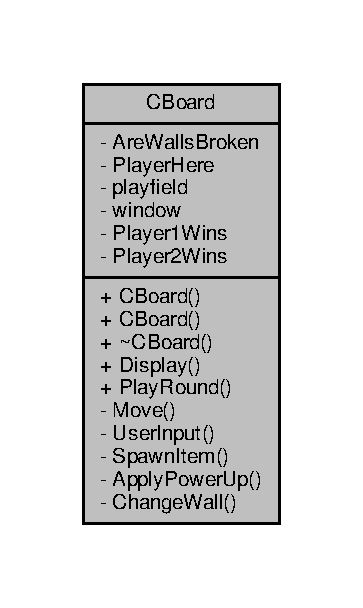
\includegraphics[width=174pt]{class_c_board__coll__graph}
\end{center}
\end{figure}
\subsection*{Public Member Functions}
\begin{DoxyCompactItemize}
\item 
\hyperlink{class_c_board_a8898bd3c57e6e91db7769a378cb3b755}{C\-Board} ()
\begin{DoxyCompactList}\small\item\em The default constructor. \end{DoxyCompactList}\item 
\hyperlink{class_c_board_a2e77f37bac4646bcf1dd6e5f24582392}{C\-Board} (\hyperlink{common_8hpp_af5a69199868671fc85779715443d7e7d}{Coor} dimensions, \hyperlink{common_8hpp_af5a69199868671fc85779715443d7e7d}{Coor} first\-Player, \hyperlink{common_8hpp_af5a69199868671fc85779715443d7e7d}{Coor} second\-Player)
\begin{DoxyCompactList}\small\item\em The detailed constructor. \end{DoxyCompactList}\item 
\hyperlink{class_c_board_a28ed0237ed02ccd928a78a7f883eb110}{$\sim$\-C\-Board} ()
\begin{DoxyCompactList}\small\item\em The destructor. \end{DoxyCompactList}\item 
void \hyperlink{class_c_board_aba95815fd50be1fe6d6c922e9c49c91c}{Display} (\hyperlink{common_8hpp_a3b27da0d46d4c36bc71511bcea2db296}{Player} current\-Round)
\begin{DoxyCompactList}\small\item\em Displays the current round of the game. \end{DoxyCompactList}\item 
bool \hyperlink{class_c_board_a9b825449509fa118303842731dde17ff}{Play\-Round} (\hyperlink{common_8hpp_a3b27da0d46d4c36bc71511bcea2db296}{Player} current\-Round, unsigned Player1\-Win\-Nb, unsigned Player2\-Win\-Nb)
\begin{DoxyCompactList}\small\item\em Plays a turn of the game. \end{DoxyCompactList}\end{DoxyCompactItemize}
\subsection*{Private Member Functions}
\begin{DoxyCompactItemize}
\item 
void \hyperlink{class_c_board_adc99d54f8a5d9ae58ef3d82cd314afb1}{Move} (\hyperlink{common_8hpp_af5a69199868671fc85779715443d7e7d}{Coor} square\-To\-Move, \hyperlink{common_8hpp_afe5d319262bda17c06308828231bd68c}{Direction} direction)
\begin{DoxyCompactList}\small\item\em Moves a square of the board. \end{DoxyCompactList}\item 
\hyperlink{common_8hpp_afe5d319262bda17c06308828231bd68c}{Direction} \hyperlink{class_c_board_a1a48e50a148927a5cf49f8261777d5fa}{User\-Input} ()
\begin{DoxyCompactList}\small\item\em Gets input from the player. \end{DoxyCompactList}\item 
void \hyperlink{class_c_board_a4095c3a98176578b2e1c478b5391eb1b}{Spawn\-Item} ()
\begin{DoxyCompactList}\small\item\em Spawns an item in the board. \end{DoxyCompactList}\item 
void \hyperlink{class_c_board_ab4117c3eab65f2cb45eb1d6ad6c26b21}{Apply\-Power\-Up} (\hyperlink{common_8hpp_a3b27da0d46d4c36bc71511bcea2db296}{Player} player, \hyperlink{common_8hpp_ab119e1d9a1ae19c7528143bf1fe16c3a}{Power\-Up} power\-Up)
\begin{DoxyCompactList}\small\item\em Apply a power\-Up on a player. \end{DoxyCompactList}\item 
\hypertarget{class_c_board_a3f41c4ac3c41c93d094c9cf0574e57d9}{void \hyperlink{class_c_board_a3f41c4ac3c41c93d094c9cf0574e57d9}{Change\-Wall} ()}\label{class_c_board_a3f41c4ac3c41c93d094c9cf0574e57d9}

\begin{DoxyCompactList}\small\item\em Delete all wall in the board and generate another board with wall. \end{DoxyCompactList}\end{DoxyCompactItemize}
\subsection*{Private Attributes}
\begin{DoxyCompactItemize}
\item 
\hypertarget{class_c_board_a1a26c9148c5db7c9770f58c9881d7232}{bool \hyperlink{class_c_board_a1a26c9148c5db7c9770f58c9881d7232}{Are\-Walls\-Broken}}\label{class_c_board_a1a26c9148c5db7c9770f58c9881d7232}

\begin{DoxyCompactList}\small\item\em Contain the information if wall has been broke. \end{DoxyCompactList}\item 
bool \hyperlink{class_c_board_a1c54c3f6d57fad2c447cbabcb66d2e29}{Player\-Here}
\begin{DoxyCompactList}\small\item\em Contain the information if the player is in the Square. \end{DoxyCompactList}\item 
\hypertarget{class_c_board_ad78413ab7d844c5826450f53e38d924a}{std\-::vector$<$ std\-::vector\\*
$<$ \hyperlink{class_c_square}{C\-Square} $>$ $>$ \hyperlink{class_c_board_ad78413ab7d844c5826450f53e38d924a}{playfield}}\label{class_c_board_ad78413ab7d844c5826450f53e38d924a}

\begin{DoxyCompactList}\small\item\em Square matrix to store the playfield. \end{DoxyCompactList}\item 
\hypertarget{class_c_board_a6dd7907777f3ea059b353006259ab8ee}{W\-I\-N\-D\-O\-W $\ast$ \hyperlink{class_c_board_a6dd7907777f3ea059b353006259ab8ee}{window}}\label{class_c_board_a6dd7907777f3ea059b353006259ab8ee}

\begin{DoxyCompactList}\small\item\em ncurses window to display the playfield. \end{DoxyCompactList}\item 
\hypertarget{class_c_board_af3a56318bcaff150a5d966cb49a93dfb}{unsigned \hyperlink{class_c_board_af3a56318bcaff150a5d966cb49a93dfb}{Player1\-Wins}}\label{class_c_board_af3a56318bcaff150a5d966cb49a93dfb}

\begin{DoxyCompactList}\small\item\em Player 1 number of wins. \end{DoxyCompactList}\item 
\hypertarget{class_c_board_a9c44eb7e2e32c9b10eac874fb3fa1bb3}{unsigned \hyperlink{class_c_board_a9c44eb7e2e32c9b10eac874fb3fa1bb3}{Player2\-Wins}}\label{class_c_board_a9c44eb7e2e32c9b10eac874fb3fa1bb3}

\begin{DoxyCompactList}\small\item\em Player 2 number of wins. \end{DoxyCompactList}\end{DoxyCompactItemize}


\subsection{Detailed Description}
The board on which the game is played. 

One Board object represents one game, it has methods to advance the state of the game or display it. 

\subsection{Constructor \& Destructor Documentation}
\hypertarget{class_c_board_a8898bd3c57e6e91db7769a378cb3b755}{\index{C\-Board@{C\-Board}!C\-Board@{C\-Board}}
\index{C\-Board@{C\-Board}!CBoard@{C\-Board}}
\subsubsection[{C\-Board}]{\setlength{\rightskip}{0pt plus 5cm}C\-Board\-::\-C\-Board (
\begin{DoxyParamCaption}
{}
\end{DoxyParamCaption}
)}}\label{class_c_board_a8898bd3c57e6e91db7769a378cb3b755}


The default constructor. 

It creates a 10x10 board with players in the upper-\/right-\/most and lower-\/left-\/most positions. It's only a delegation from the detailed constructor. \hypertarget{class_c_board_a2e77f37bac4646bcf1dd6e5f24582392}{\index{C\-Board@{C\-Board}!C\-Board@{C\-Board}}
\index{C\-Board@{C\-Board}!CBoard@{C\-Board}}
\subsubsection[{C\-Board}]{\setlength{\rightskip}{0pt plus 5cm}C\-Board\-::\-C\-Board (
\begin{DoxyParamCaption}
\item[{{\bf Coor}}]{dimensions, }
\item[{{\bf Coor}}]{first\-Player, }
\item[{{\bf Coor}}]{second\-Player}
\end{DoxyParamCaption}
)}}\label{class_c_board_a2e77f37bac4646bcf1dd6e5f24582392}


The detailed constructor. 


\begin{DoxyParams}{Parameters}
{\em dimensions} & The dimensions of the desired board. \\
\hline
{\em first\-Player} & The starting coordinates of the first player. \\
\hline
{\em second\-Player} & The starting coordinates of the second player.\\
\hline
\end{DoxyParams}
It creates a board according to the specified dimensions and will place the players if they are at a valid position. It will also initialize a ncurses window and a border accordingly. 

Here is the call graph for this function\-:
\nopagebreak
\begin{figure}[H]
\begin{center}
\leavevmode
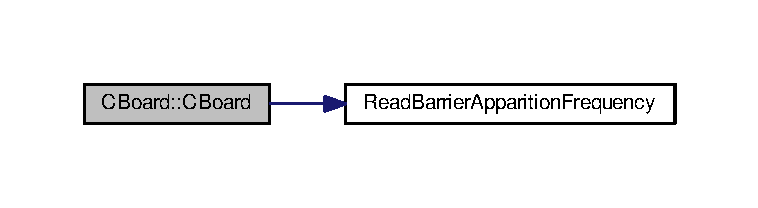
\includegraphics[width=350pt]{class_c_board_a2e77f37bac4646bcf1dd6e5f24582392_cgraph}
\end{center}
\end{figure}


\hypertarget{class_c_board_a28ed0237ed02ccd928a78a7f883eb110}{\index{C\-Board@{C\-Board}!$\sim$\-C\-Board@{$\sim$\-C\-Board}}
\index{$\sim$\-C\-Board@{$\sim$\-C\-Board}!CBoard@{C\-Board}}
\subsubsection[{$\sim$\-C\-Board}]{\setlength{\rightskip}{0pt plus 5cm}C\-Board\-::$\sim$\-C\-Board (
\begin{DoxyParamCaption}
{}
\end{DoxyParamCaption}
)}}\label{class_c_board_a28ed0237ed02ccd928a78a7f883eb110}


The destructor. 

It will get rid of the ncurses window and its border. 

\subsection{Member Function Documentation}
\hypertarget{class_c_board_ab4117c3eab65f2cb45eb1d6ad6c26b21}{\index{C\-Board@{C\-Board}!Apply\-Power\-Up@{Apply\-Power\-Up}}
\index{Apply\-Power\-Up@{Apply\-Power\-Up}!CBoard@{C\-Board}}
\subsubsection[{Apply\-Power\-Up}]{\setlength{\rightskip}{0pt plus 5cm}void C\-Board\-::\-Apply\-Power\-Up (
\begin{DoxyParamCaption}
\item[{{\bf Player}}]{player, }
\item[{{\bf Power\-Up}}]{power\-Up}
\end{DoxyParamCaption}
)\hspace{0.3cm}{\ttfamily [private]}}}\label{class_c_board_ab4117c3eab65f2cb45eb1d6ad6c26b21}


Apply a power\-Up on a player. 


\begin{DoxyParams}{Parameters}
{\em player} & the player that get the Power up \\
\hline
{\em power\-Up} & the powerup the apply \\
\hline
\end{DoxyParams}


Here is the call graph for this function\-:
\nopagebreak
\begin{figure}[H]
\begin{center}
\leavevmode
\includegraphics[width=350pt]{class_c_board_ab4117c3eab65f2cb45eb1d6ad6c26b21_cgraph}
\end{center}
\end{figure}




Here is the caller graph for this function\-:
\nopagebreak
\begin{figure}[H]
\begin{center}
\leavevmode
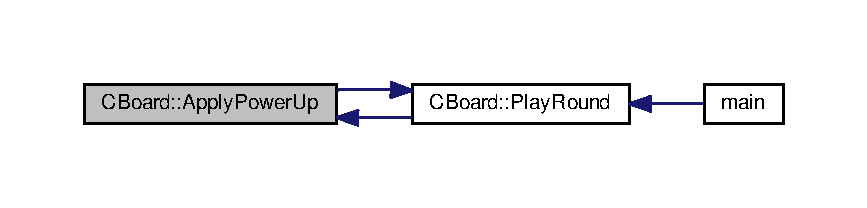
\includegraphics[width=350pt]{class_c_board_ab4117c3eab65f2cb45eb1d6ad6c26b21_icgraph}
\end{center}
\end{figure}


\hypertarget{class_c_board_aba95815fd50be1fe6d6c922e9c49c91c}{\index{C\-Board@{C\-Board}!Display@{Display}}
\index{Display@{Display}!CBoard@{C\-Board}}
\subsubsection[{Display}]{\setlength{\rightskip}{0pt plus 5cm}void C\-Board\-::\-Display (
\begin{DoxyParamCaption}
\item[{{\bf Player}}]{current\-Round}
\end{DoxyParamCaption}
)}}\label{class_c_board_aba95815fd50be1fe6d6c922e9c49c91c}


Displays the current round of the game. 


\begin{DoxyParams}{Parameters}
{\em current\-Round} & The player that will play the next turn. \\
\hline
\end{DoxyParams}


Here is the call graph for this function\-:
\nopagebreak
\begin{figure}[H]
\begin{center}
\leavevmode
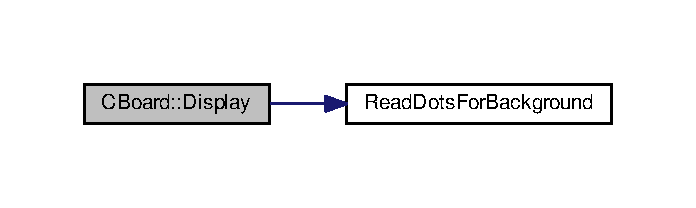
\includegraphics[width=334pt]{class_c_board_aba95815fd50be1fe6d6c922e9c49c91c_cgraph}
\end{center}
\end{figure}




Here is the caller graph for this function\-:
\nopagebreak
\begin{figure}[H]
\begin{center}
\leavevmode
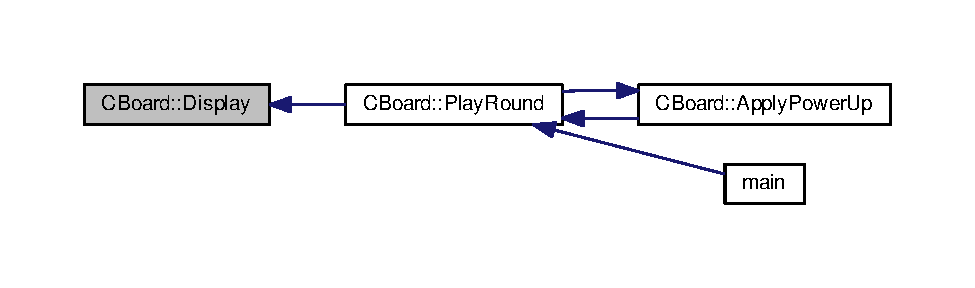
\includegraphics[width=350pt]{class_c_board_aba95815fd50be1fe6d6c922e9c49c91c_icgraph}
\end{center}
\end{figure}


\hypertarget{class_c_board_adc99d54f8a5d9ae58ef3d82cd314afb1}{\index{C\-Board@{C\-Board}!Move@{Move}}
\index{Move@{Move}!CBoard@{C\-Board}}
\subsubsection[{Move}]{\setlength{\rightskip}{0pt plus 5cm}void C\-Board\-::\-Move (
\begin{DoxyParamCaption}
\item[{{\bf Coor}}]{square\-To\-Move, }
\item[{{\bf Direction}}]{direction}
\end{DoxyParamCaption}
)\hspace{0.3cm}{\ttfamily [private]}}}\label{class_c_board_adc99d54f8a5d9ae58ef3d82cd314afb1}


Moves a square of the board. 


\begin{DoxyParams}{Parameters}
{\em square\-To\-Move} & The coordinates of the Square that will be moved. \\
\hline
{\em direction} & The Direction in which the Square will be moved.\\
\hline
\end{DoxyParams}
No check are made in the validity of the input. The Square is swapped with the one in the specified direction, its content is not modified. 

Here is the caller graph for this function\-:
\nopagebreak
\begin{figure}[H]
\begin{center}
\leavevmode
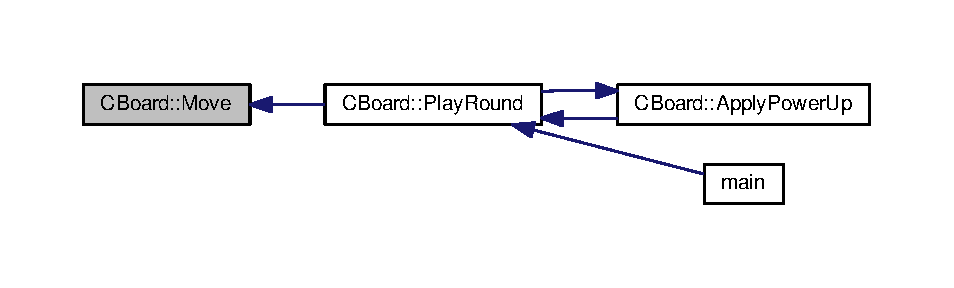
\includegraphics[width=350pt]{class_c_board_adc99d54f8a5d9ae58ef3d82cd314afb1_icgraph}
\end{center}
\end{figure}


\hypertarget{class_c_board_a9b825449509fa118303842731dde17ff}{\index{C\-Board@{C\-Board}!Play\-Round@{Play\-Round}}
\index{Play\-Round@{Play\-Round}!CBoard@{C\-Board}}
\subsubsection[{Play\-Round}]{\setlength{\rightskip}{0pt plus 5cm}bool C\-Board\-::\-Play\-Round (
\begin{DoxyParamCaption}
\item[{{\bf Player}}]{current\-Round, }
\item[{unsigned}]{Player1\-Win\-Nb, }
\item[{unsigned}]{Player2\-Win\-Nb}
\end{DoxyParamCaption}
)}}\label{class_c_board_a9b825449509fa118303842731dde17ff}


Plays a turn of the game. 


\begin{DoxyParams}{Parameters}
{\em current\-Round} & The player that will play the turn. If it is no\-\_\-player, the turn is skipped. \\
\hline
{\em Player1\-Win\-Nb} & the number of rounds won by player1. \\
\hline
{\em Player2\-Win\-Nb} & the number of rounds won by player2. \\
\hline
\end{DoxyParams}
\begin{DoxyReturn}{Returns}
true if a player moves over the other, false otherwise.
\end{DoxyReturn}
This procedure will get the input of the player until it is valid and will then move the player square accordingly. 

Here is the call graph for this function\-:
\nopagebreak
\begin{figure}[H]
\begin{center}
\leavevmode
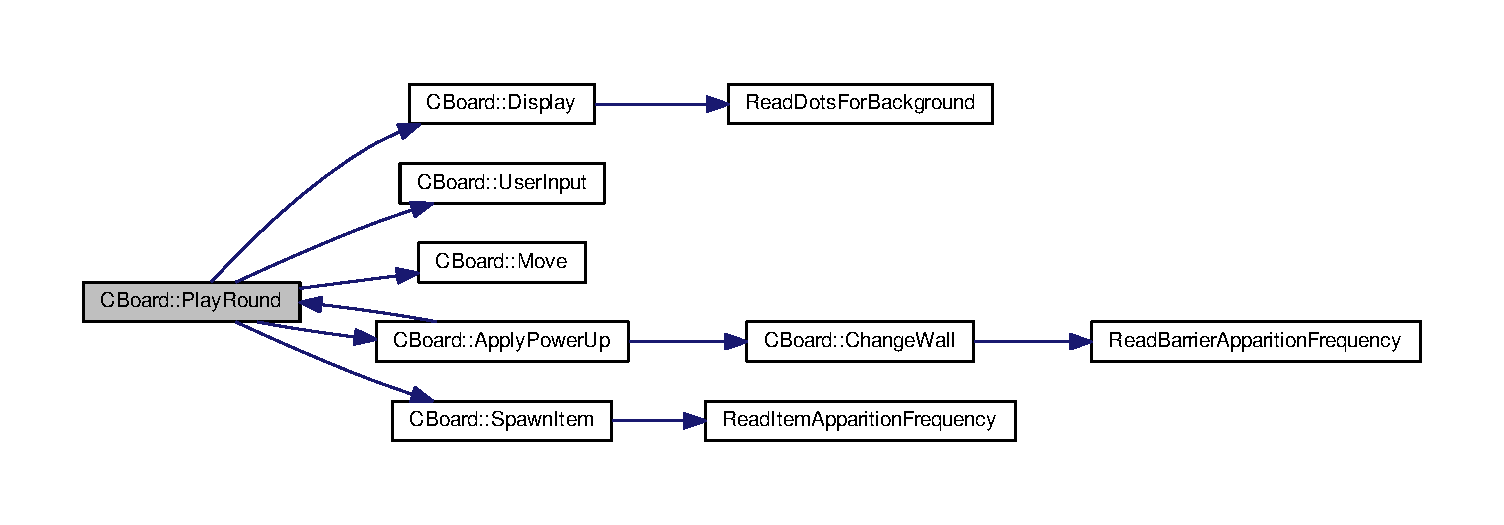
\includegraphics[width=350pt]{class_c_board_a9b825449509fa118303842731dde17ff_cgraph}
\end{center}
\end{figure}




Here is the caller graph for this function\-:
\nopagebreak
\begin{figure}[H]
\begin{center}
\leavevmode
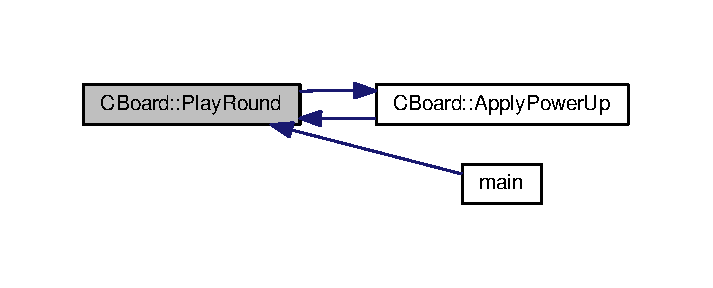
\includegraphics[width=342pt]{class_c_board_a9b825449509fa118303842731dde17ff_icgraph}
\end{center}
\end{figure}


\hypertarget{class_c_board_a4095c3a98176578b2e1c478b5391eb1b}{\index{C\-Board@{C\-Board}!Spawn\-Item@{Spawn\-Item}}
\index{Spawn\-Item@{Spawn\-Item}!CBoard@{C\-Board}}
\subsubsection[{Spawn\-Item}]{\setlength{\rightskip}{0pt plus 5cm}void C\-Board\-::\-Spawn\-Item (
\begin{DoxyParamCaption}
{}
\end{DoxyParamCaption}
)\hspace{0.3cm}{\ttfamily [private]}}}\label{class_c_board_a4095c3a98176578b2e1c478b5391eb1b}


Spawns an item in the board. 

This method will spawn an item in a free Square of the board. The frequency of spawn is variable in the setting. 

Here is the call graph for this function\-:
\nopagebreak
\begin{figure}[H]
\begin{center}
\leavevmode
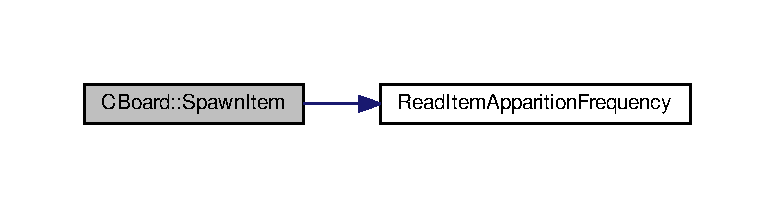
\includegraphics[width=350pt]{class_c_board_a4095c3a98176578b2e1c478b5391eb1b_cgraph}
\end{center}
\end{figure}




Here is the caller graph for this function\-:
\nopagebreak
\begin{figure}[H]
\begin{center}
\leavevmode
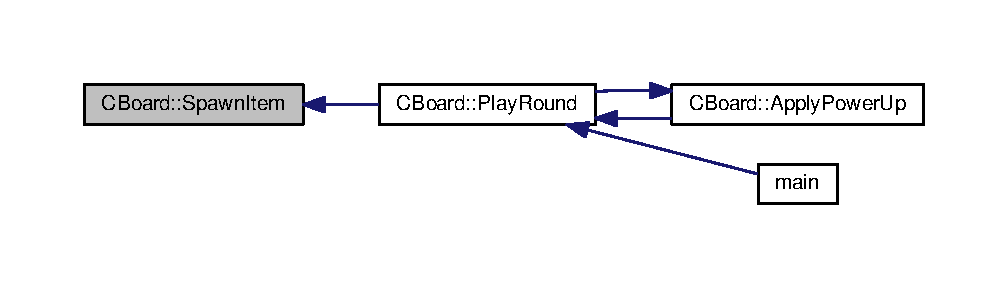
\includegraphics[width=350pt]{class_c_board_a4095c3a98176578b2e1c478b5391eb1b_icgraph}
\end{center}
\end{figure}


\hypertarget{class_c_board_a1a48e50a148927a5cf49f8261777d5fa}{\index{C\-Board@{C\-Board}!User\-Input@{User\-Input}}
\index{User\-Input@{User\-Input}!CBoard@{C\-Board}}
\subsubsection[{User\-Input}]{\setlength{\rightskip}{0pt plus 5cm}{\bf Direction} C\-Board\-::\-User\-Input (
\begin{DoxyParamCaption}
{}
\end{DoxyParamCaption}
)\hspace{0.3cm}{\ttfamily [private]}}}\label{class_c_board_a1a48e50a148927a5cf49f8261777d5fa}


Gets input from the player. 

\begin{DoxyReturn}{Returns}
The direction chosen by the user. 
\end{DoxyReturn}

\begin{DoxyExceptions}{Exceptions}
{\em \hyperlink{structuser__exit}{user\-\_\-exit}} & if the player presses E\-S\-C, resulting in the program closing successfuly. \\
\hline
\end{DoxyExceptions}


Here is the caller graph for this function\-:
\nopagebreak
\begin{figure}[H]
\begin{center}
\leavevmode
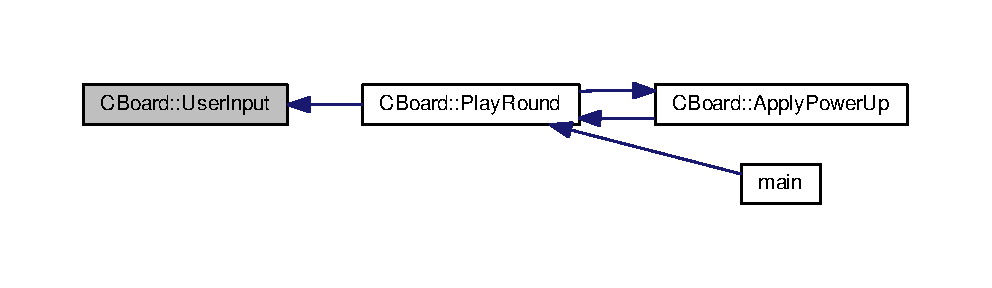
\includegraphics[width=350pt]{class_c_board_a1a48e50a148927a5cf49f8261777d5fa_icgraph}
\end{center}
\end{figure}




\subsection{Member Data Documentation}
\hypertarget{class_c_board_a1c54c3f6d57fad2c447cbabcb66d2e29}{\index{C\-Board@{C\-Board}!Player\-Here@{Player\-Here}}
\index{Player\-Here@{Player\-Here}!CBoard@{C\-Board}}
\subsubsection[{Player\-Here}]{\setlength{\rightskip}{0pt plus 5cm}bool C\-Board\-::\-Player\-Here\hspace{0.3cm}{\ttfamily [private]}}}\label{class_c_board_a1c54c3f6d57fad2c447cbabcb66d2e29}


Contain the information if the player is in the Square. 

Use only for the Double\-Speed effect. 

The documentation for this class was generated from the following files\-:\begin{DoxyCompactItemize}
\item 
src/\hyperlink{board_8hpp}{board.\-hpp}\item 
src/\hyperlink{board_8cpp}{board.\-cpp}\end{DoxyCompactItemize}

\hypertarget{class_c_form}{\section{C\-Form Class Reference}
\label{class_c_form}\index{C\-Form@{C\-Form}}
}


The form used as settings panel.  




{\ttfamily \#include $<$form.\-hpp$>$}



Collaboration diagram for C\-Form\-:
\nopagebreak
\begin{figure}[H]
\begin{center}
\leavevmode
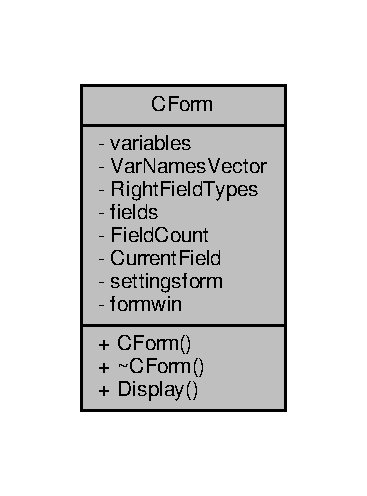
\includegraphics[width=176pt]{class_c_form__coll__graph}
\end{center}
\end{figure}
\subsection*{Public Member Functions}
\begin{DoxyCompactItemize}
\item 
\hyperlink{class_c_form_a4437c27a5eeca382ad066037381a1424}{C\-Form} (const std\-::vector$<$ std\-::string $>$ \&K\-Variable\-Names, const std\-::vector$<$ F\-I\-E\-L\-D\-T\-Y\-P\-E $\ast$ $>$ \&K\-Field\-Types, std\-::vector$<$ void $\ast$ $>$ Variables\-Values\-Pt)
\begin{DoxyCompactList}\small\item\em The constructor. \end{DoxyCompactList}\item 
\hyperlink{class_c_form_a131fd2633df654300620aafeff3e6f7f}{$\sim$\-C\-Form} ()
\begin{DoxyCompactList}\small\item\em The destructor. \end{DoxyCompactList}\item 
void \hyperlink{class_c_form_ae690ac0bad444e2ad18b6b26eb9193a5}{Display} ()
\begin{DoxyCompactList}\small\item\em Displays the setting form. \end{DoxyCompactList}\end{DoxyCompactItemize}
\subsection*{Private Attributes}
\begin{DoxyCompactItemize}
\item 
\hypertarget{class_c_form_ac2f5c5169ad400f4f5a32c65aecdd14f}{std\-::vector$<$ void $\ast$ $>$ \hyperlink{class_c_form_ac2f5c5169ad400f4f5a32c65aecdd14f}{variables}}\label{class_c_form_ac2f5c5169ad400f4f5a32c65aecdd14f}

\begin{DoxyCompactList}\small\item\em contain the values of the variables that appear in the fields \end{DoxyCompactList}\item 
\hypertarget{class_c_form_a075f201739b27a33099ac1a3fe415d87}{std\-::vector$<$ std\-::string $>$ \hyperlink{class_c_form_a075f201739b27a33099ac1a3fe415d87}{Var\-Names\-Vector}}\label{class_c_form_a075f201739b27a33099ac1a3fe415d87}

\begin{DoxyCompactList}\small\item\em contain the names of the variables that appear in the fields \end{DoxyCompactList}\item 
\hypertarget{class_c_form_a265a3dc8e13610c920f41f8ac755da0f}{std\-::vector$<$ F\-I\-E\-L\-D\-T\-Y\-P\-E $\ast$ $>$ \hyperlink{class_c_form_a265a3dc8e13610c920f41f8ac755da0f}{Right\-Field\-Types}}\label{class_c_form_a265a3dc8e13610c920f41f8ac755da0f}

\begin{DoxyCompactList}\small\item\em contain the types of the variables that appear in the fields \end{DoxyCompactList}\item 
\hypertarget{class_c_form_a9d0228604b58ba8ee4d1c2eea87bc2fe}{F\-I\-E\-L\-D $\ast$$\ast$ \hyperlink{class_c_form_a9d0228604b58ba8ee4d1c2eea87bc2fe}{fields}}\label{class_c_form_a9d0228604b58ba8ee4d1c2eea87bc2fe}

\begin{DoxyCompactList}\small\item\em the fields of the form \end{DoxyCompactList}\item 
\hypertarget{class_c_form_a66298e20d5b612661c822deef78290ad}{unsigned \hyperlink{class_c_form_a66298e20d5b612661c822deef78290ad}{Field\-Count}}\label{class_c_form_a66298e20d5b612661c822deef78290ad}

\begin{DoxyCompactList}\small\item\em the number of fields that appear in the form \end{DoxyCompactList}\item 
\hypertarget{class_c_form_adf3211c9b2d6cfb98d1d1670127abf8d}{unsigned \hyperlink{class_c_form_adf3211c9b2d6cfb98d1d1670127abf8d}{Current\-Field}}\label{class_c_form_adf3211c9b2d6cfb98d1d1670127abf8d}

\begin{DoxyCompactList}\small\item\em the indice of the current field \end{DoxyCompactList}\item 
\hypertarget{class_c_form_a47d9255ecad93a3d6e3e9ada49293d33}{F\-O\-R\-M $\ast$ \hyperlink{class_c_form_a47d9255ecad93a3d6e3e9ada49293d33}{settingsform}}\label{class_c_form_a47d9255ecad93a3d6e3e9ada49293d33}

\begin{DoxyCompactList}\small\item\em the form that contains all the fields \end{DoxyCompactList}\item 
\hypertarget{class_c_form_aa2610e56233b291cca05f56d2d7991ce}{W\-I\-N\-D\-O\-W $\ast$ \hyperlink{class_c_form_aa2610e56233b291cca05f56d2d7991ce}{formwin}}\label{class_c_form_aa2610e56233b291cca05f56d2d7991ce}

\begin{DoxyCompactList}\small\item\em the windows that will contain the form \end{DoxyCompactList}\end{DoxyCompactItemize}


\subsection{Detailed Description}
The form used as settings panel. 

The fom will generate a setting window that will enable the user to set the option as wanted. 

\subsection{Constructor \& Destructor Documentation}
\hypertarget{class_c_form_a4437c27a5eeca382ad066037381a1424}{\index{C\-Form@{C\-Form}!C\-Form@{C\-Form}}
\index{C\-Form@{C\-Form}!CForm@{C\-Form}}
\subsubsection[{C\-Form}]{\setlength{\rightskip}{0pt plus 5cm}C\-Form\-::\-C\-Form (
\begin{DoxyParamCaption}
\item[{const std\-::vector$<$ std\-::string $>$ \&}]{K\-Variable\-Names, }
\item[{const std\-::vector$<$ F\-I\-E\-L\-D\-T\-Y\-P\-E $\ast$ $>$ \&}]{K\-Field\-Types, }
\item[{std\-::vector$<$ void $\ast$ $>$}]{Variables\-Values\-Pt}
\end{DoxyParamCaption}
)}}\label{class_c_form_a4437c27a5eeca382ad066037381a1424}


The constructor. 


\begin{DoxyParams}{Parameters}
{\em K\-Variable\-Names} & The names of the variables that appear in the form. \\
\hline
{\em K\-Field\-Types} & The types of the variables that appear in the form. \\
\hline
{\em Variables\-Values\-Pt} & The values of the variables that appear in the form.\\
\hline
\end{DoxyParams}
Will create the form windows and generate all the fields according to the variables. we give in first, second and thirs place parameters. \hypertarget{class_c_form_a131fd2633df654300620aafeff3e6f7f}{\index{C\-Form@{C\-Form}!$\sim$\-C\-Form@{$\sim$\-C\-Form}}
\index{$\sim$\-C\-Form@{$\sim$\-C\-Form}!CForm@{C\-Form}}
\subsubsection[{$\sim$\-C\-Form}]{\setlength{\rightskip}{0pt plus 5cm}C\-Form\-::$\sim$\-C\-Form (
\begin{DoxyParamCaption}
{}
\end{DoxyParamCaption}
)}}\label{class_c_form_a131fd2633df654300620aafeff3e6f7f}


The destructor. 

Will free the memory the fields used and remove the W\-I\-N\-D\-O\-W. 

\subsection{Member Function Documentation}
\hypertarget{class_c_form_ae690ac0bad444e2ad18b6b26eb9193a5}{\index{C\-Form@{C\-Form}!Display@{Display}}
\index{Display@{Display}!CForm@{C\-Form}}
\subsubsection[{Display}]{\setlength{\rightskip}{0pt plus 5cm}void C\-Form\-::\-Display (
\begin{DoxyParamCaption}
{}
\end{DoxyParamCaption}
)}}\label{class_c_form_ae690ac0bad444e2ad18b6b26eb9193a5}


Displays the setting form. 

The method will diplay the setting form that the user is able to modify and will send the new values to the configuration manager. 

Here is the call graph for this function\-:
\nopagebreak
\begin{figure}[H]
\begin{center}
\leavevmode
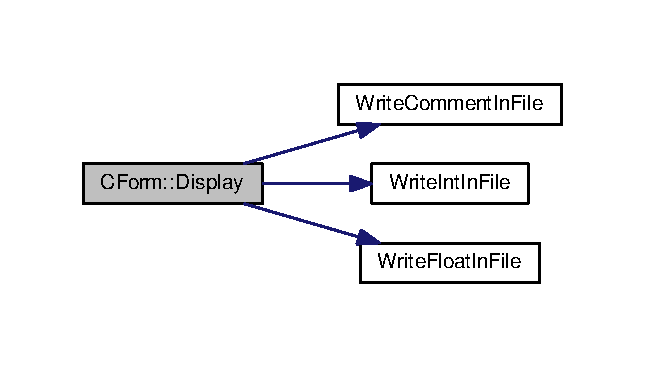
\includegraphics[width=310pt]{class_c_form_ae690ac0bad444e2ad18b6b26eb9193a5_cgraph}
\end{center}
\end{figure}




Here is the caller graph for this function\-:
\nopagebreak
\begin{figure}[H]
\begin{center}
\leavevmode
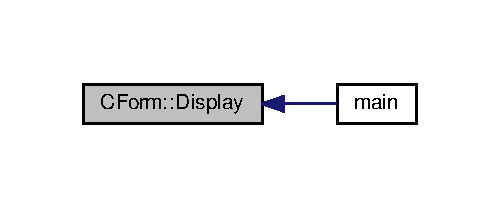
\includegraphics[width=240pt]{class_c_form_ae690ac0bad444e2ad18b6b26eb9193a5_icgraph}
\end{center}
\end{figure}




The documentation for this class was generated from the following files\-:\begin{DoxyCompactItemize}
\item 
src/\hyperlink{form_8hpp}{form.\-hpp}\item 
src/\hyperlink{form_8cpp}{form.\-cpp}\end{DoxyCompactItemize}

\hypertarget{class_c_help}{\section{C\-Help Class Reference}
\label{class_c_help}\index{C\-Help@{C\-Help}}
}


The help window.  




{\ttfamily \#include $<$help.\-hpp$>$}



Collaboration diagram for C\-Help\-:
\nopagebreak
\begin{figure}[H]
\begin{center}
\leavevmode
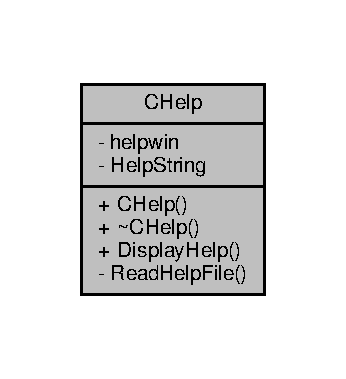
\includegraphics[width=166pt]{class_c_help__coll__graph}
\end{center}
\end{figure}
\subsection*{Public Member Functions}
\begin{DoxyCompactItemize}
\item 
\hyperlink{class_c_help_afde74ec5f76090baa26f50fc1a3a4a15}{C\-Help} ()
\begin{DoxyCompactList}\small\item\em The constructor. \end{DoxyCompactList}\item 
\hyperlink{class_c_help_ad3c627f6eaf41e7bc30d50a0f40aa0ad}{$\sim$\-C\-Help} ()
\begin{DoxyCompactList}\small\item\em The destructor. \end{DoxyCompactList}\item 
void \hyperlink{class_c_help_a48a3f3fdd8587ebd0732cfa31c27bf47}{Display\-Help} ()
\begin{DoxyCompactList}\small\item\em Displays help window. \end{DoxyCompactList}\end{DoxyCompactItemize}
\subsection*{Private Member Functions}
\begin{DoxyCompactItemize}
\item 
void \hyperlink{class_c_help_a3b274aa242a0419df9193b4bcfe798c5}{Read\-Help\-File} (const std\-::string \&K\-File\-Name)
\begin{DoxyCompactList}\small\item\em Read the help file. \end{DoxyCompactList}\end{DoxyCompactItemize}
\subsection*{Private Attributes}
\begin{DoxyCompactItemize}
\item 
\hypertarget{class_c_help_a5bb48ef48b69605b984ec9ce3d6cda21}{W\-I\-N\-D\-O\-W $\ast$ \hyperlink{class_c_help_a5bb48ef48b69605b984ec9ce3d6cda21}{helpwin}}\label{class_c_help_a5bb48ef48b69605b984ec9ce3d6cda21}

\begin{DoxyCompactList}\small\item\em The W\-I\-N\-D\-O\-W the help information are displayed into. \end{DoxyCompactList}\item 
\hypertarget{class_c_help_a0067c2eda03c1765d048bc6005a7b7eb}{std\-::string \hyperlink{class_c_help_a0067c2eda03c1765d048bc6005a7b7eb}{Help\-String}}\label{class_c_help_a0067c2eda03c1765d048bc6005a7b7eb}

\begin{DoxyCompactList}\small\item\em The string the information contained in the help file are stored into. \end{DoxyCompactList}\end{DoxyCompactItemize}


\subsection{Detailed Description}
The help window. 

The help is the window that will show help to the user about how to play the game and about how the cofiguration file was made. 

\subsection{Constructor \& Destructor Documentation}
\hypertarget{class_c_help_afde74ec5f76090baa26f50fc1a3a4a15}{\index{C\-Help@{C\-Help}!C\-Help@{C\-Help}}
\index{C\-Help@{C\-Help}!CHelp@{C\-Help}}
\subsubsection[{C\-Help}]{\setlength{\rightskip}{0pt plus 5cm}C\-Help\-::\-C\-Help (
\begin{DoxyParamCaption}
{}
\end{DoxyParamCaption}
)}}\label{class_c_help_afde74ec5f76090baa26f50fc1a3a4a15}


The constructor. 

The constructor will generate the window and read the help file to display. 

Here is the call graph for this function\-:
\nopagebreak
\begin{figure}[H]
\begin{center}
\leavevmode
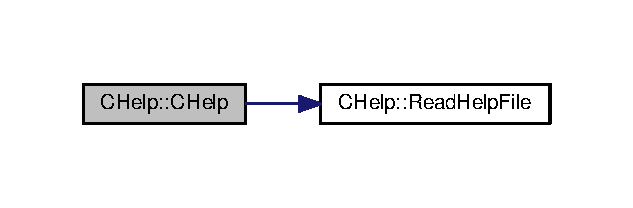
\includegraphics[width=304pt]{class_c_help_afde74ec5f76090baa26f50fc1a3a4a15_cgraph}
\end{center}
\end{figure}


\hypertarget{class_c_help_ad3c627f6eaf41e7bc30d50a0f40aa0ad}{\index{C\-Help@{C\-Help}!$\sim$\-C\-Help@{$\sim$\-C\-Help}}
\index{$\sim$\-C\-Help@{$\sim$\-C\-Help}!CHelp@{C\-Help}}
\subsubsection[{$\sim$\-C\-Help}]{\setlength{\rightskip}{0pt plus 5cm}C\-Help\-::$\sim$\-C\-Help (
\begin{DoxyParamCaption}
{}
\end{DoxyParamCaption}
)}}\label{class_c_help_ad3c627f6eaf41e7bc30d50a0f40aa0ad}


The destructor. 

It will free the memory allocated by the constructor and remove the window. 

\subsection{Member Function Documentation}
\hypertarget{class_c_help_a48a3f3fdd8587ebd0732cfa31c27bf47}{\index{C\-Help@{C\-Help}!Display\-Help@{Display\-Help}}
\index{Display\-Help@{Display\-Help}!CHelp@{C\-Help}}
\subsubsection[{Display\-Help}]{\setlength{\rightskip}{0pt plus 5cm}void C\-Help\-::\-Display\-Help (
\begin{DoxyParamCaption}
{}
\end{DoxyParamCaption}
)}}\label{class_c_help_a48a3f3fdd8587ebd0732cfa31c27bf47}


Displays help window. 

The function will open a new window that will display the informations the player needs to play. It contains commands, the rules of the game and the available options in the configuration file. 

Here is the caller graph for this function\-:
\nopagebreak
\begin{figure}[H]
\begin{center}
\leavevmode
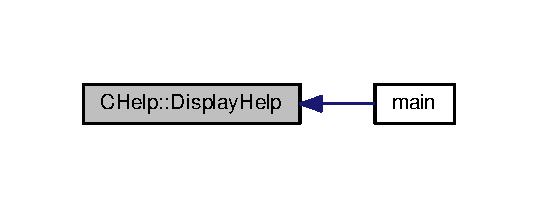
\includegraphics[width=258pt]{class_c_help_a48a3f3fdd8587ebd0732cfa31c27bf47_icgraph}
\end{center}
\end{figure}


\hypertarget{class_c_help_a3b274aa242a0419df9193b4bcfe798c5}{\index{C\-Help@{C\-Help}!Read\-Help\-File@{Read\-Help\-File}}
\index{Read\-Help\-File@{Read\-Help\-File}!CHelp@{C\-Help}}
\subsubsection[{Read\-Help\-File}]{\setlength{\rightskip}{0pt plus 5cm}void C\-Help\-::\-Read\-Help\-File (
\begin{DoxyParamCaption}
\item[{const std\-::string \&}]{K\-File\-Name}
\end{DoxyParamCaption}
)\hspace{0.3cm}{\ttfamily [private]}}}\label{class_c_help_a3b274aa242a0419df9193b4bcfe798c5}


Read the help file. 


\begin{DoxyParams}{Parameters}
{\em K\-File\-Name} & The path of the help file.\\
\hline
\end{DoxyParams}
The function will read the help file that have the path we give by parameters and store the file in a vector. 

Here is the caller graph for this function\-:
\nopagebreak
\begin{figure}[H]
\begin{center}
\leavevmode
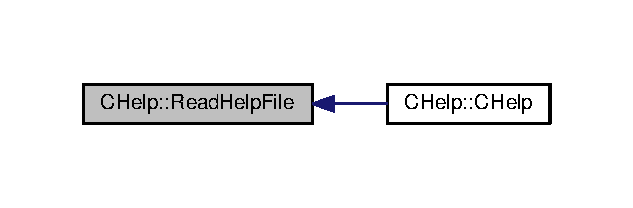
\includegraphics[width=304pt]{class_c_help_a3b274aa242a0419df9193b4bcfe798c5_icgraph}
\end{center}
\end{figure}




The documentation for this class was generated from the following files\-:\begin{DoxyCompactItemize}
\item 
src/\hyperlink{help_8hpp}{help.\-hpp}\item 
src/\hyperlink{help_8cpp}{help.\-cpp}\end{DoxyCompactItemize}

\hypertarget{class_c_menu}{\section{C\-Menu Class Reference}
\label{class_c_menu}\index{C\-Menu@{C\-Menu}}
}


A user-\/friendly menu.  




{\ttfamily \#include $<$menu.\-hpp$>$}



Collaboration diagram for C\-Menu\-:
\nopagebreak
\begin{figure}[H]
\begin{center}
\leavevmode
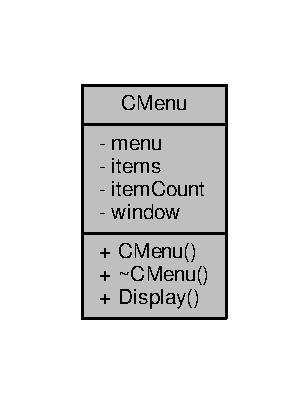
\includegraphics[width=148pt]{class_c_menu__coll__graph}
\end{center}
\end{figure}
\subsection*{Public Member Functions}
\begin{DoxyCompactItemize}
\item 
\hyperlink{class_c_menu_a8b1ad64c4215258c64d0e5d5a622ba76}{C\-Menu} (std\-::vector$<$ std\-::string $>$ choices)
\begin{DoxyCompactList}\small\item\em The constructor. \end{DoxyCompactList}\item 
\hyperlink{class_c_menu_ab2ab7e24e646bcb61ad0b9d8484f2604}{$\sim$\-C\-Menu} ()
\begin{DoxyCompactList}\small\item\em The destructor. \end{DoxyCompactList}\item 
std\-::string \hyperlink{class_c_menu_a6cc86670a0f6bfc0ac9a97d938226b5c}{Display} ()
\begin{DoxyCompactList}\small\item\em Displays the menu window and returns the choice of the user. \end{DoxyCompactList}\end{DoxyCompactItemize}
\subsection*{Private Attributes}
\begin{DoxyCompactItemize}
\item 
\hypertarget{class_c_menu_a33e0e8d76b9a003fa92bd542f5111c3c}{M\-E\-N\-U $\ast$ \hyperlink{class_c_menu_a33e0e8d76b9a003fa92bd542f5111c3c}{menu}}\label{class_c_menu_a33e0e8d76b9a003fa92bd542f5111c3c}

\begin{DoxyCompactList}\small\item\em A pointer to the ncurses M\-E\-N\-U used by the Menu. \end{DoxyCompactList}\item 
\hypertarget{class_c_menu_ab5471bd4a9ade3600f6cf58f1220011a}{I\-T\-E\-M $\ast$$\ast$ \hyperlink{class_c_menu_ab5471bd4a9ade3600f6cf58f1220011a}{items}}\label{class_c_menu_ab5471bd4a9ade3600f6cf58f1220011a}

\begin{DoxyCompactList}\small\item\em A pointer to an array of the I\-T\-E\-Ms used by the M\-E\-N\-U. \end{DoxyCompactList}\item 
unsigned \hyperlink{class_c_menu_a4903eda2d318231beca52dac4373fda6}{item\-Count}
\begin{DoxyCompactList}\small\item\em The number of elements of the array items points to. \end{DoxyCompactList}\item 
\hypertarget{class_c_menu_a0d6c0c7f61a72ec9d8dd0957c5240887}{W\-I\-N\-D\-O\-W $\ast$ \hyperlink{class_c_menu_a0d6c0c7f61a72ec9d8dd0957c5240887}{window}}\label{class_c_menu_a0d6c0c7f61a72ec9d8dd0957c5240887}

\begin{DoxyCompactList}\small\item\em The W\-I\-N\-D\-O\-W the menu is displayed into. \end{DoxyCompactList}\end{DoxyCompactItemize}


\subsection{Detailed Description}
A user-\/friendly menu. 

A Menu object lets the user choose between different options with arrow keys. The Menu class uses directly the M\-E\-N\-U type from ncurses as defined in menu.\-h 

\subsection{Constructor \& Destructor Documentation}
\hypertarget{class_c_menu_a8b1ad64c4215258c64d0e5d5a622ba76}{\index{C\-Menu@{C\-Menu}!C\-Menu@{C\-Menu}}
\index{C\-Menu@{C\-Menu}!CMenu@{C\-Menu}}
\subsubsection[{C\-Menu}]{\setlength{\rightskip}{0pt plus 5cm}C\-Menu\-::\-C\-Menu (
\begin{DoxyParamCaption}
\item[{std\-::vector$<$ std\-::string $>$}]{choices}
\end{DoxyParamCaption}
)}}\label{class_c_menu_a8b1ad64c4215258c64d0e5d5a622ba76}


The constructor. 


\begin{DoxyParams}{Parameters}
{\em choices} & A vector of all the different choices the user can make.\\
\hline
\end{DoxyParams}
It will create the window the menu is displayed into and allocate the memory used to store the menu. \hypertarget{class_c_menu_ab2ab7e24e646bcb61ad0b9d8484f2604}{\index{C\-Menu@{C\-Menu}!$\sim$\-C\-Menu@{$\sim$\-C\-Menu}}
\index{$\sim$\-C\-Menu@{$\sim$\-C\-Menu}!CMenu@{C\-Menu}}
\subsubsection[{$\sim$\-C\-Menu}]{\setlength{\rightskip}{0pt plus 5cm}C\-Menu\-::$\sim$\-C\-Menu (
\begin{DoxyParamCaption}
{}
\end{DoxyParamCaption}
)}}\label{class_c_menu_ab2ab7e24e646bcb61ad0b9d8484f2604}


The destructor. 

It will free the memory allocated by the constructor and remove the window. 

\subsection{Member Function Documentation}
\hypertarget{class_c_menu_a6cc86670a0f6bfc0ac9a97d938226b5c}{\index{C\-Menu@{C\-Menu}!Display@{Display}}
\index{Display@{Display}!CMenu@{C\-Menu}}
\subsubsection[{Display}]{\setlength{\rightskip}{0pt plus 5cm}std\-::string C\-Menu\-::\-Display (
\begin{DoxyParamCaption}
{}
\end{DoxyParamCaption}
)}}\label{class_c_menu_a6cc86670a0f6bfc0ac9a97d938226b5c}


Displays the menu window and returns the choice of the user. 

\begin{DoxyReturn}{Returns}
The choice of the user. 
\end{DoxyReturn}


Here is the caller graph for this function\-:
\nopagebreak
\begin{figure}[H]
\begin{center}
\leavevmode
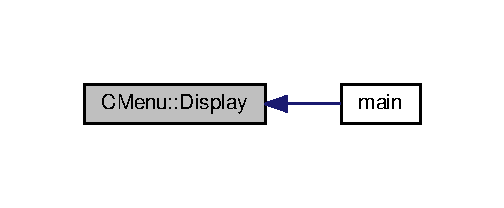
\includegraphics[width=242pt]{class_c_menu_a6cc86670a0f6bfc0ac9a97d938226b5c_icgraph}
\end{center}
\end{figure}




\subsection{Member Data Documentation}
\hypertarget{class_c_menu_a4903eda2d318231beca52dac4373fda6}{\index{C\-Menu@{C\-Menu}!item\-Count@{item\-Count}}
\index{item\-Count@{item\-Count}!CMenu@{C\-Menu}}
\subsubsection[{item\-Count}]{\setlength{\rightskip}{0pt plus 5cm}unsigned C\-Menu\-::item\-Count\hspace{0.3cm}{\ttfamily [private]}}}\label{class_c_menu_a4903eda2d318231beca52dac4373fda6}


The number of elements of the array items points to. 

This is necessary for proper destruction of the object. 

The documentation for this class was generated from the following files\-:\begin{DoxyCompactItemize}
\item 
src/\hyperlink{menu_8hpp}{menu.\-hpp}\item 
src/\hyperlink{menu_8cpp}{menu.\-cpp}\end{DoxyCompactItemize}

\hypertarget{class_c_square}{\section{C\-Square Class Reference}
\label{class_c_square}\index{C\-Square@{C\-Square}}
}


The squares of the board.  




{\ttfamily \#include $<$square.\-hpp$>$}



Collaboration diagram for C\-Square\-:
\nopagebreak
\begin{figure}[H]
\begin{center}
\leavevmode
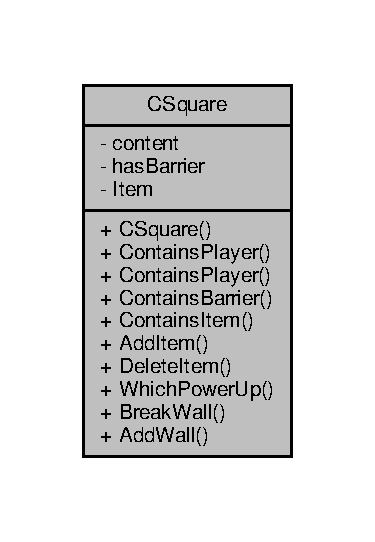
\includegraphics[width=180pt]{class_c_square__coll__graph}
\end{center}
\end{figure}
\subsection*{Public Member Functions}
\begin{DoxyCompactItemize}
\item 
\hyperlink{class_c_square_a4bbe681a17a8bc59817bd5e45d832ca2}{C\-Square} (\hyperlink{common_8hpp_a3b27da0d46d4c36bc71511bcea2db296}{Player} \hyperlink{class_c_square_ac8b1e1733091b86c3c1fedfa73a1ef11}{content}=no\-\_\-player, bool \hyperlink{class_c_square_a32454efe4a8f4ac87fbc9868306560e2}{has\-Barrier}=false)
\begin{DoxyCompactList}\small\item\em The constructor. \end{DoxyCompactList}\item 
bool \hyperlink{class_c_square_a618612b48dff26cbe8197f2371d6c78e}{Contains\-Player} ()
\begin{DoxyCompactList}\small\item\em Checks if the Square contains any player. \end{DoxyCompactList}\item 
bool \hyperlink{class_c_square_a1c2b3e4c631dd711bf34899d52f8d081}{Contains\-Player} (\hyperlink{common_8hpp_a3b27da0d46d4c36bc71511bcea2db296}{Player} p)
\begin{DoxyCompactList}\small\item\em Checks if the Square contains a particular player. \end{DoxyCompactList}\item 
bool \hyperlink{class_c_square_a983368c041402ea321b39a30e1a4c71a}{Contains\-Barrier} ()
\begin{DoxyCompactList}\small\item\em Checks if the Square contains a barrier. \end{DoxyCompactList}\item 
bool \hyperlink{class_c_square_aee8e014954d295f0e73e3170f36866a9}{Contains\-Item} ()
\begin{DoxyCompactList}\small\item\em Checks if the Square contains an item. \end{DoxyCompactList}\item 
void \hyperlink{class_c_square_ab65d8ba292e16113b67a17bdaa85ce46}{Add\-Item} (\hyperlink{common_8hpp_ab119e1d9a1ae19c7528143bf1fe16c3a}{Power\-Up} item\-To\-Add)
\begin{DoxyCompactList}\small\item\em Adds an item to the Square. \end{DoxyCompactList}\item 
\hypertarget{class_c_square_a168e70962e8656c6c01045c48928b882}{void \hyperlink{class_c_square_a168e70962e8656c6c01045c48928b882}{Delete\-Item} ()}\label{class_c_square_a168e70962e8656c6c01045c48928b882}

\begin{DoxyCompactList}\small\item\em Removes the item in the Square. \end{DoxyCompactList}\item 
\hypertarget{class_c_square_a0bb1e16bf604445de2b8c52df64bf54f}{\hyperlink{common_8hpp_ab119e1d9a1ae19c7528143bf1fe16c3a}{Power\-Up} \hyperlink{class_c_square_a0bb1e16bf604445de2b8c52df64bf54f}{Which\-Power\-Up} ()}\label{class_c_square_a0bb1e16bf604445de2b8c52df64bf54f}

\begin{DoxyCompactList}\small\item\em Checks which Power\-Up the player have. \end{DoxyCompactList}\item 
\hypertarget{class_c_square_a2b72de0d1083323b80c8cd58374b3d22}{void \hyperlink{class_c_square_a2b72de0d1083323b80c8cd58374b3d22}{Break\-Wall} ()}\label{class_c_square_a2b72de0d1083323b80c8cd58374b3d22}

\begin{DoxyCompactList}\small\item\em Removes barrier from the Square. \end{DoxyCompactList}\item 
\hypertarget{class_c_square_a30a296e4d6dfa209b5036ebfee16968a}{void \hyperlink{class_c_square_a30a296e4d6dfa209b5036ebfee16968a}{Add\-Wall} ()}\label{class_c_square_a30a296e4d6dfa209b5036ebfee16968a}

\begin{DoxyCompactList}\small\item\em Adds barrier to the Square. \end{DoxyCompactList}\end{DoxyCompactItemize}
\subsection*{Private Attributes}
\begin{DoxyCompactItemize}
\item 
\hypertarget{class_c_square_ac8b1e1733091b86c3c1fedfa73a1ef11}{\hyperlink{common_8hpp_a3b27da0d46d4c36bc71511bcea2db296}{Player} \hyperlink{class_c_square_ac8b1e1733091b86c3c1fedfa73a1ef11}{content}}\label{class_c_square_ac8b1e1733091b86c3c1fedfa73a1ef11}

\begin{DoxyCompactList}\small\item\em The content of the Square. \end{DoxyCompactList}\item 
\hypertarget{class_c_square_a32454efe4a8f4ac87fbc9868306560e2}{bool \hyperlink{class_c_square_a32454efe4a8f4ac87fbc9868306560e2}{has\-Barrier}}\label{class_c_square_a32454efe4a8f4ac87fbc9868306560e2}

\begin{DoxyCompactList}\small\item\em Stores if the Square contains a barrier. \end{DoxyCompactList}\item 
\hypertarget{class_c_square_a696d7dc5495225e9f48e982b3e0b221c}{\hyperlink{common_8hpp_ab119e1d9a1ae19c7528143bf1fe16c3a}{Power\-Up} \hyperlink{class_c_square_a696d7dc5495225e9f48e982b3e0b221c}{Item}}\label{class_c_square_a696d7dc5495225e9f48e982b3e0b221c}

\begin{DoxyCompactList}\small\item\em Stores the kind of item the Square contains. \end{DoxyCompactList}\end{DoxyCompactItemize}


\subsection{Detailed Description}
The squares of the board. 

One Square object represents one square of the playfield and its content. The content of a Square cannot be modified after its creation. 

\subsection{Constructor \& Destructor Documentation}
\hypertarget{class_c_square_a4bbe681a17a8bc59817bd5e45d832ca2}{\index{C\-Square@{C\-Square}!C\-Square@{C\-Square}}
\index{C\-Square@{C\-Square}!CSquare@{C\-Square}}
\subsubsection[{C\-Square}]{\setlength{\rightskip}{0pt plus 5cm}C\-Square\-::\-C\-Square (
\begin{DoxyParamCaption}
\item[{{\bf Player}}]{content = {\ttfamily no\-\_\-player}, }
\item[{bool}]{has\-Barrier = {\ttfamily false}}
\end{DoxyParamCaption}
)}}\label{class_c_square_a4bbe681a17a8bc59817bd5e45d832ca2}


The constructor. 


\begin{DoxyParams}{Parameters}
{\em content} & The content of the Square, defaults to no\-\_\-player. \\
\hline
{\em has\-Barrier} & Specifies if the Square contains a barrier, default to false. \\
\hline
\end{DoxyParams}


\subsection{Member Function Documentation}
\hypertarget{class_c_square_ab65d8ba292e16113b67a17bdaa85ce46}{\index{C\-Square@{C\-Square}!Add\-Item@{Add\-Item}}
\index{Add\-Item@{Add\-Item}!CSquare@{C\-Square}}
\subsubsection[{Add\-Item}]{\setlength{\rightskip}{0pt plus 5cm}void C\-Square\-::\-Add\-Item (
\begin{DoxyParamCaption}
\item[{{\bf Power\-Up}}]{item\-To\-Add}
\end{DoxyParamCaption}
)}}\label{class_c_square_ab65d8ba292e16113b67a17bdaa85ce46}


Adds an item to the Square. 


\begin{DoxyParams}{Parameters}
{\em item\-To\-Add} & The item to add to the Square. \\
\hline
\end{DoxyParams}
\hypertarget{class_c_square_a983368c041402ea321b39a30e1a4c71a}{\index{C\-Square@{C\-Square}!Contains\-Barrier@{Contains\-Barrier}}
\index{Contains\-Barrier@{Contains\-Barrier}!CSquare@{C\-Square}}
\subsubsection[{Contains\-Barrier}]{\setlength{\rightskip}{0pt plus 5cm}bool C\-Square\-::\-Contains\-Barrier (
\begin{DoxyParamCaption}
{}
\end{DoxyParamCaption}
)}}\label{class_c_square_a983368c041402ea321b39a30e1a4c71a}


Checks if the Square contains a barrier. 

\begin{DoxyReturn}{Returns}
true if the Square contains a barrier, false otherwise. 
\end{DoxyReturn}
\hypertarget{class_c_square_aee8e014954d295f0e73e3170f36866a9}{\index{C\-Square@{C\-Square}!Contains\-Item@{Contains\-Item}}
\index{Contains\-Item@{Contains\-Item}!CSquare@{C\-Square}}
\subsubsection[{Contains\-Item}]{\setlength{\rightskip}{0pt plus 5cm}bool C\-Square\-::\-Contains\-Item (
\begin{DoxyParamCaption}
{}
\end{DoxyParamCaption}
)}}\label{class_c_square_aee8e014954d295f0e73e3170f36866a9}


Checks if the Square contains an item. 

\begin{DoxyReturn}{Returns}
true if the Square contains an item, false otherwise. 
\end{DoxyReturn}
\hypertarget{class_c_square_a618612b48dff26cbe8197f2371d6c78e}{\index{C\-Square@{C\-Square}!Contains\-Player@{Contains\-Player}}
\index{Contains\-Player@{Contains\-Player}!CSquare@{C\-Square}}
\subsubsection[{Contains\-Player}]{\setlength{\rightskip}{0pt plus 5cm}bool C\-Square\-::\-Contains\-Player (
\begin{DoxyParamCaption}
{}
\end{DoxyParamCaption}
)}}\label{class_c_square_a618612b48dff26cbe8197f2371d6c78e}


Checks if the Square contains any player. 

\begin{DoxyReturn}{Returns}
false if the Square contains no\-\_\-player, true otherwise. 
\end{DoxyReturn}
\hypertarget{class_c_square_a1c2b3e4c631dd711bf34899d52f8d081}{\index{C\-Square@{C\-Square}!Contains\-Player@{Contains\-Player}}
\index{Contains\-Player@{Contains\-Player}!CSquare@{C\-Square}}
\subsubsection[{Contains\-Player}]{\setlength{\rightskip}{0pt plus 5cm}bool C\-Square\-::\-Contains\-Player (
\begin{DoxyParamCaption}
\item[{{\bf Player}}]{p}
\end{DoxyParamCaption}
)}}\label{class_c_square_a1c2b3e4c631dd711bf34899d52f8d081}


Checks if the Square contains a particular player. 


\begin{DoxyParams}{Parameters}
{\em p} & The player to look for. \\
\hline
\end{DoxyParams}
\begin{DoxyReturn}{Returns}
true if the Square contains p, false otherwise. 
\end{DoxyReturn}


The documentation for this class was generated from the following files\-:\begin{DoxyCompactItemize}
\item 
src/\hyperlink{square_8hpp}{square.\-hpp}\item 
src/\hyperlink{square_8cpp}{square.\-cpp}\end{DoxyCompactItemize}

\hypertarget{structuser__exit}{\section{user\-\_\-exit Struct Reference}
\label{structuser__exit}\index{user\-\_\-exit@{user\-\_\-exit}}
}


The exception type thrown when the user wants to exit the game prematurely.  




{\ttfamily \#include $<$common.\-hpp$>$}



Collaboration diagram for user\-\_\-exit\-:
\nopagebreak
\begin{figure}[H]
\begin{center}
\leavevmode
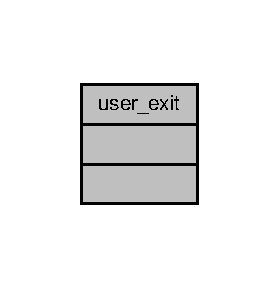
\includegraphics[width=134pt]{structuser__exit__coll__graph}
\end{center}
\end{figure}


\subsection{Detailed Description}
The exception type thrown when the user wants to exit the game prematurely. 

The documentation for this struct was generated from the following file\-:\begin{DoxyCompactItemize}
\item 
src/\hyperlink{common_8hpp}{common.\-hpp}\end{DoxyCompactItemize}

\chapter{File Documentation}
\hypertarget{board_8cpp}{\section{src/board.cpp File Reference}
\label{board_8cpp}\index{src/board.\-cpp@{src/board.\-cpp}}
}


Board class implementation.  


{\ttfamily \#include \char`\"{}board.\-hpp\char`\"{}}\\*
Include dependency graph for board.\-cpp\-:
\nopagebreak
\begin{figure}[H]
\begin{center}
\leavevmode
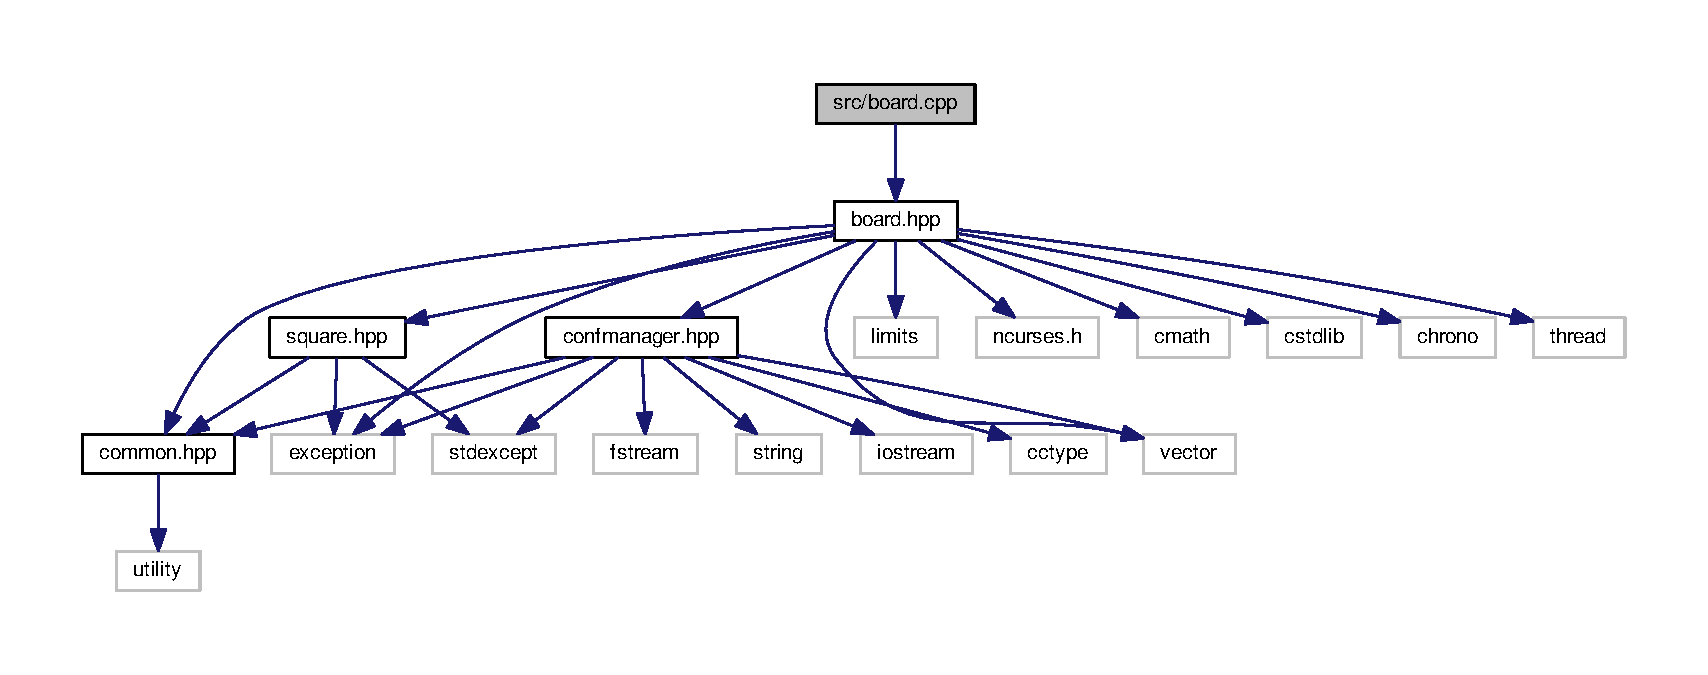
\includegraphics[width=350pt]{board_8cpp__incl}
\end{center}
\end{figure}


\subsection{Detailed Description}
Board class implementation. \begin{DoxyAuthor}{Authors}
\-: J. Saffi, Y. Vidal, Y. Roux, A. Torres Aurora Dugo
\end{DoxyAuthor}
\begin{DoxyDate}{Date}
\-: 08/01/14
\end{DoxyDate}
\begin{DoxyVersion}{Version}
\-: 1.\-0
\end{DoxyVersion}
\begin{DoxySeeAlso}{See Also}
\hyperlink{board_8hpp}{board.\-hpp} 
\end{DoxySeeAlso}

\hypertarget{board_8hpp}{\section{src/board.hpp File Reference}
\label{board_8hpp}\index{src/board.\-hpp@{src/board.\-hpp}}
}


Board class header.  


{\ttfamily \#include \char`\"{}common.\-hpp\char`\"{}}\\*
{\ttfamily \#include \char`\"{}square.\-hpp\char`\"{}}\\*
{\ttfamily \#include \char`\"{}confmanager.\-hpp\char`\"{}}\\*
{\ttfamily \#include $<$vector$>$}\\*
{\ttfamily \#include $<$limits$>$}\\*
{\ttfamily \#include $<$exception$>$}\\*
{\ttfamily \#include $<$ncurses.\-h$>$}\\*
{\ttfamily \#include $<$cmath$>$}\\*
{\ttfamily \#include $<$cstdlib$>$}\\*
{\ttfamily \#include $<$chrono$>$}\\*
{\ttfamily \#include $<$thread$>$}\\*
Include dependency graph for board.\-hpp\-:
\nopagebreak
\begin{figure}[H]
\begin{center}
\leavevmode
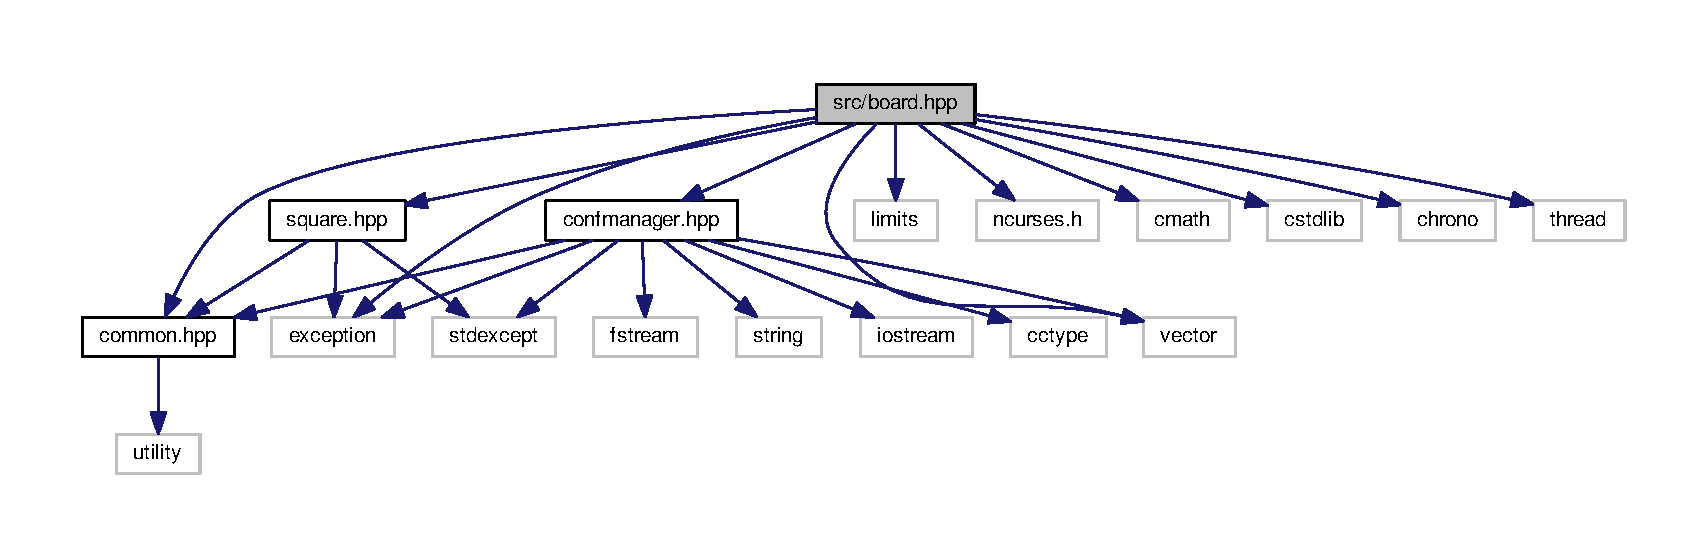
\includegraphics[width=350pt]{board_8hpp__incl}
\end{center}
\end{figure}
This graph shows which files directly or indirectly include this file\-:
\nopagebreak
\begin{figure}[H]
\begin{center}
\leavevmode
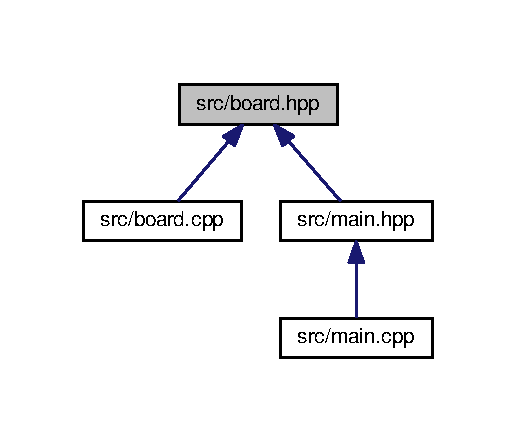
\includegraphics[width=247pt]{board_8hpp__dep__incl}
\end{center}
\end{figure}
\subsection*{Classes}
\begin{DoxyCompactItemize}
\item 
class \hyperlink{class_c_board}{C\-Board}
\begin{DoxyCompactList}\small\item\em The board on which the game is played. \end{DoxyCompactList}\end{DoxyCompactItemize}


\subsection{Detailed Description}
Board class header. \begin{DoxyAuthor}{Authors}
\-: J. Saffi, Y. Vidal, Y. Roux, A. Torres Aurora Dugo
\end{DoxyAuthor}
\begin{DoxyDate}{Date}
\-: 08/01/14
\end{DoxyDate}
\begin{DoxyVersion}{Version}
\-: 1.\-0
\end{DoxyVersion}
\begin{DoxySeeAlso}{See Also}
\hyperlink{board_8cpp}{board.\-cpp} 
\end{DoxySeeAlso}

\hypertarget{common_8hpp}{\section{src/common.hpp File Reference}
\label{common_8hpp}\index{src/common.\-hpp@{src/common.\-hpp}}
}


Common header.  


{\ttfamily \#include $<$utility$>$}\\*
Include dependency graph for common.\-hpp\-:
\nopagebreak
\begin{figure}[H]
\begin{center}
\leavevmode
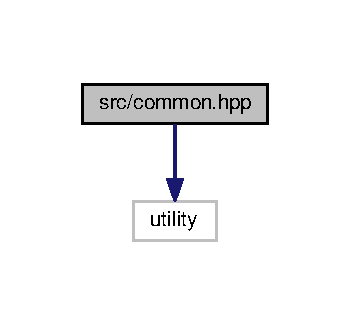
\includegraphics[width=168pt]{common_8hpp__incl}
\end{center}
\end{figure}
This graph shows which files directly or indirectly include this file\-:
\nopagebreak
\begin{figure}[H]
\begin{center}
\leavevmode
\includegraphics[width=350pt]{common_8hpp__dep__incl}
\end{center}
\end{figure}
\subsection*{Classes}
\begin{DoxyCompactItemize}
\item 
struct \hyperlink{structuser__exit}{user\-\_\-exit}
\begin{DoxyCompactList}\small\item\em The exception type thrown when the user wants to exit the game prematurely. \end{DoxyCompactList}\end{DoxyCompactItemize}
\subsection*{Typedefs}
\begin{DoxyCompactItemize}
\item 
\hypertarget{common_8hpp_af5a69199868671fc85779715443d7e7d}{typedef std\-::pair$<$ unsigned, \\*
unsigned $>$ \hyperlink{common_8hpp_af5a69199868671fc85779715443d7e7d}{Coor}}\label{common_8hpp_af5a69199868671fc85779715443d7e7d}

\begin{DoxyCompactList}\small\item\em Coordinates in a two dimensionnal matrix. \end{DoxyCompactList}\end{DoxyCompactItemize}
\subsection*{Enumerations}
\begin{DoxyCompactItemize}
\item 
enum \hyperlink{common_8hpp_a3b27da0d46d4c36bc71511bcea2db296}{Player} \{ {\bfseries player1} = 1, 
{\bfseries player2} = 2, 
{\bfseries no\-\_\-player} = 3
 \}
\begin{DoxyCompactList}\small\item\em One of the players or no\-\_\-player. \end{DoxyCompactList}\item 
enum \hyperlink{common_8hpp_afe5d319262bda17c06308828231bd68c}{Direction} \{ \\*
{\bfseries north}, 
{\bfseries north\-\_\-east}, 
{\bfseries east}, 
{\bfseries south\-\_\-east}, 
\\*
{\bfseries south}, 
{\bfseries south\-\_\-west}, 
{\bfseries west}, 
{\bfseries north\-\_\-west}
 \}
\begin{DoxyCompactList}\small\item\em One of the eight cardinal points. \end{DoxyCompactList}\item 
enum \hyperlink{common_8hpp_ab119e1d9a1ae19c7528143bf1fe16c3a}{Power\-Up} \{ \\*
{\bfseries double\-\_\-speed}, 
{\bfseries teleportation}, 
{\bfseries break\-\_\-wall}, 
{\bfseries change\-\_\-wall}, 
\\*
{\bfseries no\-\_\-power\-\_\-up}
 \}
\begin{DoxyCompactList}\small\item\em Different sort of power up. \end{DoxyCompactList}\end{DoxyCompactItemize}


\subsection{Detailed Description}
Common header. \begin{DoxyAuthor}{Authors}
\-: J. Saffi, Y. Vidal, Y. Roux, A. Torres Aurora Dugo
\end{DoxyAuthor}
\begin{DoxyDate}{Date}
\-: 08/01/14
\end{DoxyDate}
\begin{DoxyVersion}{Version}
\-: 1.\-0
\end{DoxyVersion}
Contains the type definitions used throughout the project.

\begin{DoxySeeAlso}{See Also}
\hyperlink{board_8cpp}{board.\-cpp} 
\end{DoxySeeAlso}

\hypertarget{confmanager_8cpp}{\section{src/confmanager.cpp File Reference}
\label{confmanager_8cpp}\index{src/confmanager.\-cpp@{src/confmanager.\-cpp}}
}


Configuration file management implementation.  


{\ttfamily \#include \char`\"{}confmanager.\-hpp\char`\"{}}\\*
{\ttfamily \#include $<$iomanip$>$}\\*
Include dependency graph for confmanager.\-cpp\-:
\nopagebreak
\begin{figure}[H]
\begin{center}
\leavevmode
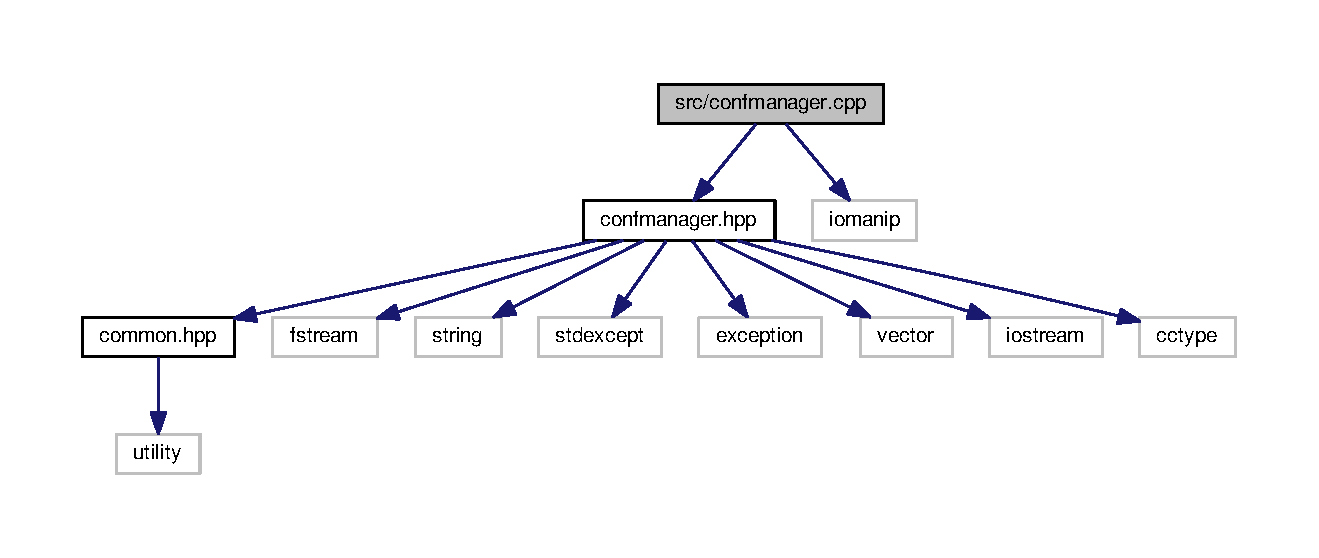
\includegraphics[width=350pt]{confmanager_8cpp__incl}
\end{center}
\end{figure}
\subsection*{Functions}
\begin{DoxyCompactItemize}
\item 
{\footnotesize template$<$typename T\-Y\-P\-E $>$ }\\T\-Y\-P\-E \hyperlink{confmanager_8cpp_a6d1b57352b5ac61eabdabed63da30e8c}{Read\-Variable} (const std\-::string \&K\-File\-Name, const std\-::string \&K\-Variable\-Name)
\begin{DoxyCompactList}\small\item\em Configuration file parser for one variable. \end{DoxyCompactList}\item 
{\footnotesize template$<$typename T\-Y\-P\-E $>$ }\\void \hyperlink{confmanager_8cpp_a5ff71d17cc5ab971ba56b1da5c2bd4b4}{Write\-Variable} (const std\-::string \&K\-File\-Name, const std\-::string \&K\-Variable\-Name, const T\-Y\-P\-E \&K\-Variable\-Value, bool Erase\-File)
\begin{DoxyCompactList}\small\item\em Configuration file writer for one variable. \end{DoxyCompactList}\item 
\hyperlink{common_8hpp_a3b27da0d46d4c36bc71511bcea2db296}{Player} \hyperlink{confmanager_8cpp_a7320e0a28c46c1cf87e5b1e37c4d118f}{Read\-Starting\-Player} ()
\begin{DoxyCompactList}\small\item\em Reads the starting Player in the config file. \end{DoxyCompactList}\item 
\hyperlink{common_8hpp_af5a69199868671fc85779715443d7e7d}{Coor} \hyperlink{confmanager_8cpp_a21454348fa3ef45b2521b40eccb565c1}{Read\-Board\-Dimensions} ()
\begin{DoxyCompactList}\small\item\em Reads the dimensions of the board in the config file. \end{DoxyCompactList}\item 
int \hyperlink{confmanager_8cpp_abed3527c8a74d39e07eca9b02fd76e4f}{Read\-Player\-Color} (\hyperlink{common_8hpp_a3b27da0d46d4c36bc71511bcea2db296}{Player} player)
\begin{DoxyCompactList}\small\item\em Reads the player color in the config file. \end{DoxyCompactList}\item 
int \hyperlink{confmanager_8cpp_ae91dc572702641134500948058bbfd8d}{Read\-Item\-Color} ()
\begin{DoxyCompactList}\small\item\em Reads the item color in the config file. \end{DoxyCompactList}\item 
float \hyperlink{confmanager_8cpp_ab932d580893f474c2b6964224a611956}{Read\-Barrier\-Apparition\-Frequency} ()
\begin{DoxyCompactList}\small\item\em Reads the apparition frequency of barriers. \end{DoxyCompactList}\item 
float \hyperlink{confmanager_8cpp_aea31b5d159b5351035176535e4abb7d8}{Read\-Item\-Apparition\-Frequency} ()
\begin{DoxyCompactList}\small\item\em Reads the apparition frequency of items. \end{DoxyCompactList}\item 
bool \hyperlink{confmanager_8cpp_a3d49b8db3f20fb5a3dbca93f7a08e59a}{Read\-Dots\-For\-Background} ()
\begin{DoxyCompactList}\small\item\em Read if the background display dots or not. \end{DoxyCompactList}\item 
void \hyperlink{confmanager_8cpp_a1d7e449f88cd4b8f3f304bffedff4cf8}{Write\-Float\-In\-File} (const std\-::string \&K\-Variable\-Name, char $\ast$Variable\-Value)
\begin{DoxyCompactList}\small\item\em Write a float number in the configuration file. \end{DoxyCompactList}\item 
void \hyperlink{confmanager_8cpp_aa77d65a36d86e37926c1c3accd5bcd4f}{Write\-Int\-In\-File} (const std\-::string \&K\-Variable\-Name, char $\ast$Variable\-Value)
\begin{DoxyCompactList}\small\item\em Write an integer number in the configuration file. \end{DoxyCompactList}\item 
void \hyperlink{confmanager_8cpp_ade5d04a2a7fde153840d5a0748f3f0a7}{Write\-Comment\-In\-File} (const std\-::string \&K\-Comment, bool Erase\-File)
\begin{DoxyCompactList}\small\item\em Write a comment in the configuration file. \end{DoxyCompactList}\end{DoxyCompactItemize}


\subsection{Detailed Description}
Configuration file management implementation. \begin{DoxyAuthor}{Authors}
\-: J. Saffi, Y. Vidal, Y. Roux, A. Torres Aurora Dugo
\end{DoxyAuthor}
\begin{DoxyDate}{Date}
\-: 08/01/14
\end{DoxyDate}
\begin{DoxyVersion}{Version}
\-: 1.\-0
\end{DoxyVersion}
\begin{DoxySeeAlso}{See Also}
\hyperlink{confmanager_8hpp}{confmanager.\-hpp} 
\end{DoxySeeAlso}


\subsection{Function Documentation}
\hypertarget{confmanager_8cpp_ab932d580893f474c2b6964224a611956}{\index{confmanager.\-cpp@{confmanager.\-cpp}!Read\-Barrier\-Apparition\-Frequency@{Read\-Barrier\-Apparition\-Frequency}}
\index{Read\-Barrier\-Apparition\-Frequency@{Read\-Barrier\-Apparition\-Frequency}!confmanager.cpp@{confmanager.\-cpp}}
\subsubsection[{Read\-Barrier\-Apparition\-Frequency}]{\setlength{\rightskip}{0pt plus 5cm}Read\-Barrier\-Apparition\-Frequency (
\begin{DoxyParamCaption}
{}
\end{DoxyParamCaption}
)}}\label{confmanager_8cpp_ab932d580893f474c2b6964224a611956}


Reads the apparition frequency of barriers. 

\begin{DoxyReturn}{Returns}
The apparition frequency of barriers.
\end{DoxyReturn}
The returned value is between 0 and 1. 

Here is the caller graph for this function\-:
\nopagebreak
\begin{figure}[H]
\begin{center}
\leavevmode
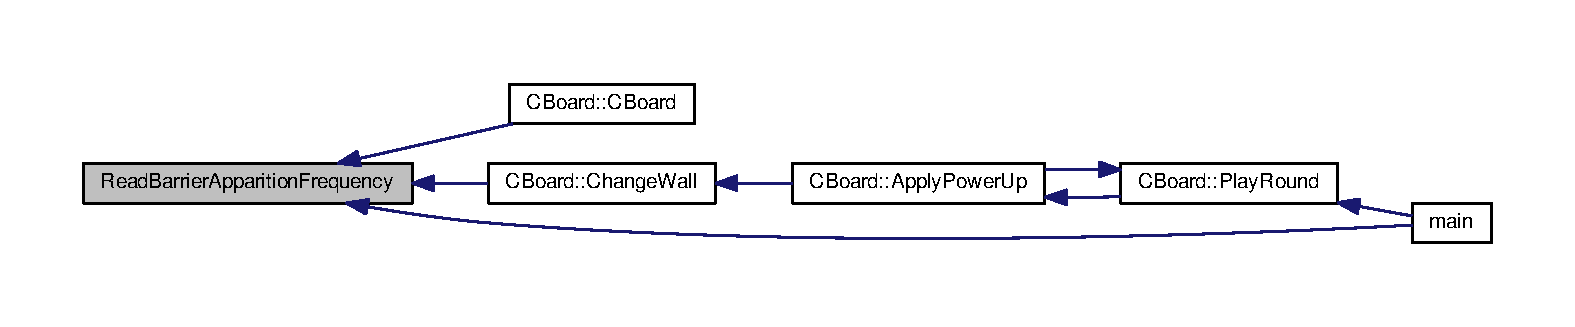
\includegraphics[width=350pt]{confmanager_8cpp_ab932d580893f474c2b6964224a611956_icgraph}
\end{center}
\end{figure}


\hypertarget{confmanager_8cpp_a21454348fa3ef45b2521b40eccb565c1}{\index{confmanager.\-cpp@{confmanager.\-cpp}!Read\-Board\-Dimensions@{Read\-Board\-Dimensions}}
\index{Read\-Board\-Dimensions@{Read\-Board\-Dimensions}!confmanager.cpp@{confmanager.\-cpp}}
\subsubsection[{Read\-Board\-Dimensions}]{\setlength{\rightskip}{0pt plus 5cm}{\bf Coor} Read\-Board\-Dimensions (
\begin{DoxyParamCaption}
{}
\end{DoxyParamCaption}
)}}\label{confmanager_8cpp_a21454348fa3ef45b2521b40eccb565c1}


Reads the dimensions of the board in the config file. 

\begin{DoxyReturn}{Returns}
The dimensions of the board.
\end{DoxyReturn}
The function will return the dimensions of the board as set in the configuration file. It uses the Read\-Variable function. The path of the config file is specified in a define made in \hyperlink{confmanager_8hpp}{confmanager.\-hpp} 

Here is the caller graph for this function\-:
\nopagebreak
\begin{figure}[H]
\begin{center}
\leavevmode
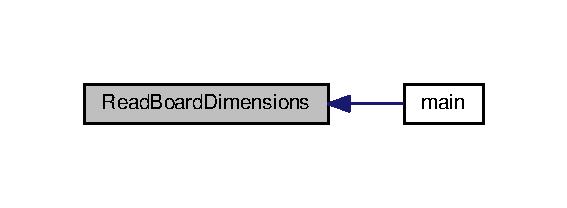
\includegraphics[width=272pt]{confmanager_8cpp_a21454348fa3ef45b2521b40eccb565c1_icgraph}
\end{center}
\end{figure}


\hypertarget{confmanager_8cpp_a3d49b8db3f20fb5a3dbca93f7a08e59a}{\index{confmanager.\-cpp@{confmanager.\-cpp}!Read\-Dots\-For\-Background@{Read\-Dots\-For\-Background}}
\index{Read\-Dots\-For\-Background@{Read\-Dots\-For\-Background}!confmanager.cpp@{confmanager.\-cpp}}
\subsubsection[{Read\-Dots\-For\-Background}]{\setlength{\rightskip}{0pt plus 5cm}Read\-Dots\-For\-Background (
\begin{DoxyParamCaption}
{}
\end{DoxyParamCaption}
)}}\label{confmanager_8cpp_a3d49b8db3f20fb5a3dbca93f7a08e59a}


Read if the background display dots or not. 

\begin{DoxyReturn}{Returns}
If the background has dots or not.
\end{DoxyReturn}
The returned value is a booleen that will set the background character to none or dots. 

Here is the caller graph for this function\-:
\nopagebreak
\begin{figure}[H]
\begin{center}
\leavevmode
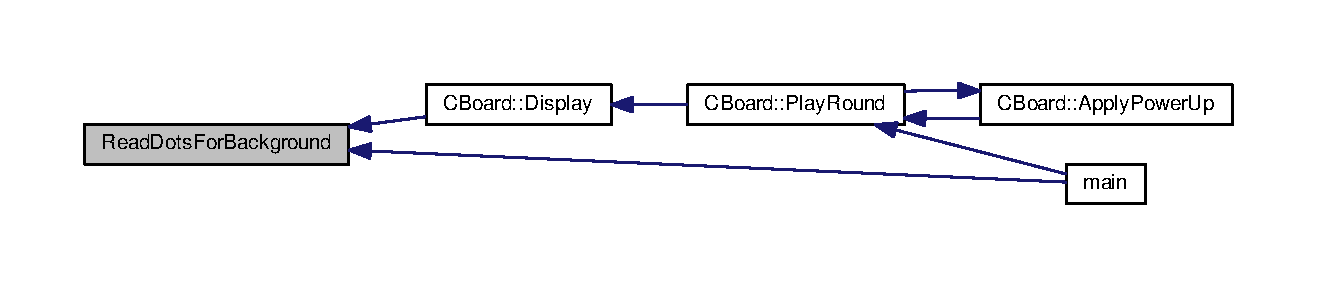
\includegraphics[width=350pt]{confmanager_8cpp_a3d49b8db3f20fb5a3dbca93f7a08e59a_icgraph}
\end{center}
\end{figure}


\hypertarget{confmanager_8cpp_aea31b5d159b5351035176535e4abb7d8}{\index{confmanager.\-cpp@{confmanager.\-cpp}!Read\-Item\-Apparition\-Frequency@{Read\-Item\-Apparition\-Frequency}}
\index{Read\-Item\-Apparition\-Frequency@{Read\-Item\-Apparition\-Frequency}!confmanager.cpp@{confmanager.\-cpp}}
\subsubsection[{Read\-Item\-Apparition\-Frequency}]{\setlength{\rightskip}{0pt plus 5cm}Read\-Item\-Apparition\-Frequency (
\begin{DoxyParamCaption}
{}
\end{DoxyParamCaption}
)}}\label{confmanager_8cpp_aea31b5d159b5351035176535e4abb7d8}


Reads the apparition frequency of items. 

\begin{DoxyReturn}{Returns}
The apparition frequency of items.
\end{DoxyReturn}
The returned value is between 0 and 1. 

Here is the caller graph for this function\-:
\nopagebreak
\begin{figure}[H]
\begin{center}
\leavevmode
\includegraphics[width=350pt]{confmanager_8cpp_aea31b5d159b5351035176535e4abb7d8_icgraph}
\end{center}
\end{figure}


\hypertarget{confmanager_8cpp_ae91dc572702641134500948058bbfd8d}{\index{confmanager.\-cpp@{confmanager.\-cpp}!Read\-Item\-Color@{Read\-Item\-Color}}
\index{Read\-Item\-Color@{Read\-Item\-Color}!confmanager.cpp@{confmanager.\-cpp}}
\subsubsection[{Read\-Item\-Color}]{\setlength{\rightskip}{0pt plus 5cm}int Read\-Item\-Color (
\begin{DoxyParamCaption}
{}
\end{DoxyParamCaption}
)}}\label{confmanager_8cpp_ae91dc572702641134500948058bbfd8d}


Reads the item color in the config file. 

\begin{DoxyReturn}{Returns}
The Item's color equivalent as an ncurses define.
\end{DoxyReturn}
It uses the Read\-Variable function to read the configuration file. The path of the config file is specified in a define made in \hyperlink{confmanager_8hpp}{confmanager.\-hpp} 

Here is the caller graph for this function\-:
\nopagebreak
\begin{figure}[H]
\begin{center}
\leavevmode
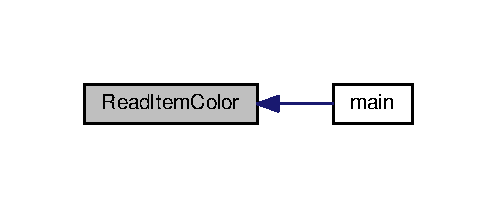
\includegraphics[width=238pt]{confmanager_8cpp_ae91dc572702641134500948058bbfd8d_icgraph}
\end{center}
\end{figure}


\hypertarget{confmanager_8cpp_abed3527c8a74d39e07eca9b02fd76e4f}{\index{confmanager.\-cpp@{confmanager.\-cpp}!Read\-Player\-Color@{Read\-Player\-Color}}
\index{Read\-Player\-Color@{Read\-Player\-Color}!confmanager.cpp@{confmanager.\-cpp}}
\subsubsection[{Read\-Player\-Color}]{\setlength{\rightskip}{0pt plus 5cm}int Read\-Player\-Color (
\begin{DoxyParamCaption}
\item[{{\bf Player}}]{player}
\end{DoxyParamCaption}
)}}\label{confmanager_8cpp_abed3527c8a74d39e07eca9b02fd76e4f}


Reads the player color in the config file. 


\begin{DoxyParams}{Parameters}
{\em player} & Player to get the color of. \\
\hline
\end{DoxyParams}
\begin{DoxyReturn}{Returns}
The Player's color equivalent as an ncurses define.
\end{DoxyReturn}
The function will return the color of the player whose name is the parameter. It uses the Read\-Variable function to read the configuration file. The path of the config file is specified in a define made in \hyperlink{confmanager_8hpp}{confmanager.\-hpp} 

Here is the caller graph for this function\-:
\nopagebreak
\begin{figure}[H]
\begin{center}
\leavevmode
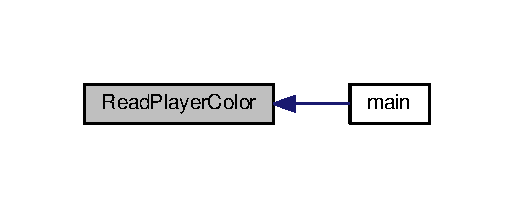
\includegraphics[width=246pt]{confmanager_8cpp_abed3527c8a74d39e07eca9b02fd76e4f_icgraph}
\end{center}
\end{figure}


\hypertarget{confmanager_8cpp_a7320e0a28c46c1cf87e5b1e37c4d118f}{\index{confmanager.\-cpp@{confmanager.\-cpp}!Read\-Starting\-Player@{Read\-Starting\-Player}}
\index{Read\-Starting\-Player@{Read\-Starting\-Player}!confmanager.cpp@{confmanager.\-cpp}}
\subsubsection[{Read\-Starting\-Player}]{\setlength{\rightskip}{0pt plus 5cm}{\bf Player} Read\-Starting\-Player (
\begin{DoxyParamCaption}
{}
\end{DoxyParamCaption}
)}}\label{confmanager_8cpp_a7320e0a28c46c1cf87e5b1e37c4d118f}


Reads the starting Player in the config file. 

\begin{DoxyReturn}{Returns}
The starting Player.
\end{DoxyReturn}
The function will return which player will begin to play. It uses the Read\-Variable Function. The path of the config file is specified in a define made in \hyperlink{confmanager_8hpp}{confmanager.\-hpp} 

Here is the caller graph for this function\-:
\nopagebreak
\begin{figure}[H]
\begin{center}
\leavevmode
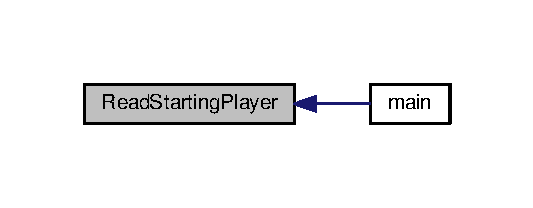
\includegraphics[width=256pt]{confmanager_8cpp_a7320e0a28c46c1cf87e5b1e37c4d118f_icgraph}
\end{center}
\end{figure}


\hypertarget{confmanager_8cpp_a6d1b57352b5ac61eabdabed63da30e8c}{\index{confmanager.\-cpp@{confmanager.\-cpp}!Read\-Variable@{Read\-Variable}}
\index{Read\-Variable@{Read\-Variable}!confmanager.cpp@{confmanager.\-cpp}}
\subsubsection[{Read\-Variable}]{\setlength{\rightskip}{0pt plus 5cm}template$<$typename T\-Y\-P\-E $>$ template$<$ typename T\-Y\-P\-E $>$ T\-Y\-P\-E Read\-Variable (
\begin{DoxyParamCaption}
\item[{const std\-::string \&}]{K\-File\-Name, }
\item[{const std\-::string \&}]{K\-Variable\-Name}
\end{DoxyParamCaption}
)}}\label{confmanager_8cpp_a6d1b57352b5ac61eabdabed63da30e8c}


Configuration file parser for one variable. 


\begin{DoxyParams}{Parameters}
{\em K\-File\-Name} & File path of the configuration file. \\
\hline
{\em K\-Variable\-Name} & Name of the parsed variable. \\
\hline
\end{DoxyParams}
\begin{DoxyReturn}{Returns}
The parsed value of the variable.
\end{DoxyReturn}
The function will parse the file we give him in first place parameter. To achieve this, it will read the variable's value in the configuration file and return the value. It uses a template to be able to parse any type using operator $>$$>$ \hypertarget{confmanager_8cpp_ade5d04a2a7fde153840d5a0748f3f0a7}{\index{confmanager.\-cpp@{confmanager.\-cpp}!Write\-Comment\-In\-File@{Write\-Comment\-In\-File}}
\index{Write\-Comment\-In\-File@{Write\-Comment\-In\-File}!confmanager.cpp@{confmanager.\-cpp}}
\subsubsection[{Write\-Comment\-In\-File}]{\setlength{\rightskip}{0pt plus 5cm}void Write\-Comment\-In\-File (
\begin{DoxyParamCaption}
\item[{const std\-::string \&}]{K\-Comment, }
\item[{bool}]{Erase\-File = {\ttfamily false}}
\end{DoxyParamCaption}
)}}\label{confmanager_8cpp_ade5d04a2a7fde153840d5a0748f3f0a7}


Write a comment in the configuration file. 


\begin{DoxyParams}{Parameters}
{\em K\-Comment} & The comment to inject. \\
\hline
{\em Erase\-File} & Set if the configuration file have to be erased.\\
\hline
\end{DoxyParams}
The function will write the the comment gave in parameters thanks to the Write\-Variable template 

Here is the caller graph for this function\-:
\nopagebreak
\begin{figure}[H]
\begin{center}
\leavevmode
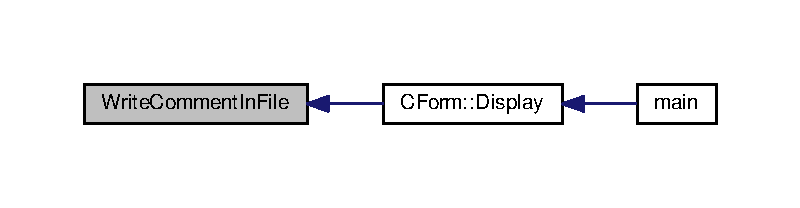
\includegraphics[width=350pt]{confmanager_8cpp_ade5d04a2a7fde153840d5a0748f3f0a7_icgraph}
\end{center}
\end{figure}


\hypertarget{confmanager_8cpp_a1d7e449f88cd4b8f3f304bffedff4cf8}{\index{confmanager.\-cpp@{confmanager.\-cpp}!Write\-Float\-In\-File@{Write\-Float\-In\-File}}
\index{Write\-Float\-In\-File@{Write\-Float\-In\-File}!confmanager.cpp@{confmanager.\-cpp}}
\subsubsection[{Write\-Float\-In\-File}]{\setlength{\rightskip}{0pt plus 5cm}void Write\-Float\-In\-File (
\begin{DoxyParamCaption}
\item[{const std\-::string \&}]{K\-Variable\-Name, }
\item[{char $\ast$}]{Variable\-Value}
\end{DoxyParamCaption}
)}}\label{confmanager_8cpp_a1d7e449f88cd4b8f3f304bffedff4cf8}


Write a float number in the configuration file. 


\begin{DoxyParams}{Parameters}
{\em K\-Variable\-Name} & The name of the variable to inject. \\
\hline
{\em Variable\-Value} & The value of the variable to inject.\\
\hline
\end{DoxyParams}
The function will write the name of the float variable and her value thanks to the Write\-Variable template. 

Here is the caller graph for this function\-:
\nopagebreak
\begin{figure}[H]
\begin{center}
\leavevmode
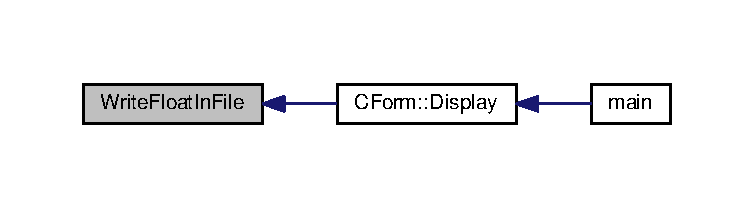
\includegraphics[width=350pt]{confmanager_8cpp_a1d7e449f88cd4b8f3f304bffedff4cf8_icgraph}
\end{center}
\end{figure}


\hypertarget{confmanager_8cpp_aa77d65a36d86e37926c1c3accd5bcd4f}{\index{confmanager.\-cpp@{confmanager.\-cpp}!Write\-Int\-In\-File@{Write\-Int\-In\-File}}
\index{Write\-Int\-In\-File@{Write\-Int\-In\-File}!confmanager.cpp@{confmanager.\-cpp}}
\subsubsection[{Write\-Int\-In\-File}]{\setlength{\rightskip}{0pt plus 5cm}void Write\-Int\-In\-File (
\begin{DoxyParamCaption}
\item[{const std\-::string \&}]{K\-Variable\-Name, }
\item[{char $\ast$}]{Variable\-Value}
\end{DoxyParamCaption}
)}}\label{confmanager_8cpp_aa77d65a36d86e37926c1c3accd5bcd4f}


Write an integer number in the configuration file. 


\begin{DoxyParams}{Parameters}
{\em K\-Variable\-Name} & Name of the variable to inject. \\
\hline
{\em Variable\-Value} & Value of the variable to inject.\\
\hline
\end{DoxyParams}
The function will write the name of the integer variable and her value thanks to the Write\-Variable template. 

Here is the caller graph for this function\-:
\nopagebreak
\begin{figure}[H]
\begin{center}
\leavevmode
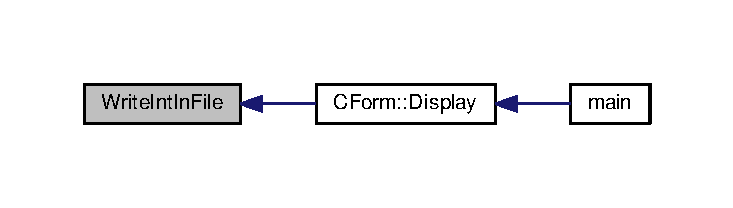
\includegraphics[width=350pt]{confmanager_8cpp_aa77d65a36d86e37926c1c3accd5bcd4f_icgraph}
\end{center}
\end{figure}


\hypertarget{confmanager_8cpp_a5ff71d17cc5ab971ba56b1da5c2bd4b4}{\index{confmanager.\-cpp@{confmanager.\-cpp}!Write\-Variable@{Write\-Variable}}
\index{Write\-Variable@{Write\-Variable}!confmanager.cpp@{confmanager.\-cpp}}
\subsubsection[{Write\-Variable}]{\setlength{\rightskip}{0pt plus 5cm}template$<$typename T\-Y\-P\-E $>$ template$<$ typename T\-Y\-P\-E $>$ void Write\-Variable (
\begin{DoxyParamCaption}
\item[{const std\-::string \&}]{K\-File\-Name, }
\item[{const std\-::string \&}]{K\-Variable\-Name, }
\item[{const T\-Y\-P\-E \&}]{K\-Variable\-Value, }
\item[{bool}]{Erase\-File}
\end{DoxyParamCaption}
)}}\label{confmanager_8cpp_a5ff71d17cc5ab971ba56b1da5c2bd4b4}


Configuration file writer for one variable. 


\begin{DoxyParams}{Parameters}
{\em K\-File\-Name} & File path of the configuration file. \\
\hline
{\em K\-Variable\-Name} & Name of the variable to inject. \\
\hline
{\em K\-Variable\-Value} & Value of the variable to inject. \\
\hline
{\em Erase\-File} & Set if the file must be erased before being writed.\\
\hline
\end{DoxyParams}
The function will write the file we give him in first place parameter and her value we give in second place parameter. To achieve this, it will write the variable and then value in the configuration file. It uses a template to be able to write any type properly using operator $>$$>$ 
\hypertarget{confmanager_8hpp}{\section{src/confmanager.hpp File Reference}
\label{confmanager_8hpp}\index{src/confmanager.\-hpp@{src/confmanager.\-hpp}}
}


Configuration file management header.  


{\ttfamily \#include \char`\"{}common.\-hpp\char`\"{}}\\*
{\ttfamily \#include $<$fstream$>$}\\*
{\ttfamily \#include $<$string$>$}\\*
{\ttfamily \#include $<$stdexcept$>$}\\*
{\ttfamily \#include $<$exception$>$}\\*
{\ttfamily \#include $<$vector$>$}\\*
{\ttfamily \#include $<$iostream$>$}\\*
{\ttfamily \#include $<$cctype$>$}\\*
Include dependency graph for confmanager.\-hpp\-:
\nopagebreak
\begin{figure}[H]
\begin{center}
\leavevmode
\includegraphics[width=350pt]{confmanager_8hpp__incl}
\end{center}
\end{figure}
This graph shows which files directly or indirectly include this file\-:
\nopagebreak
\begin{figure}[H]
\begin{center}
\leavevmode
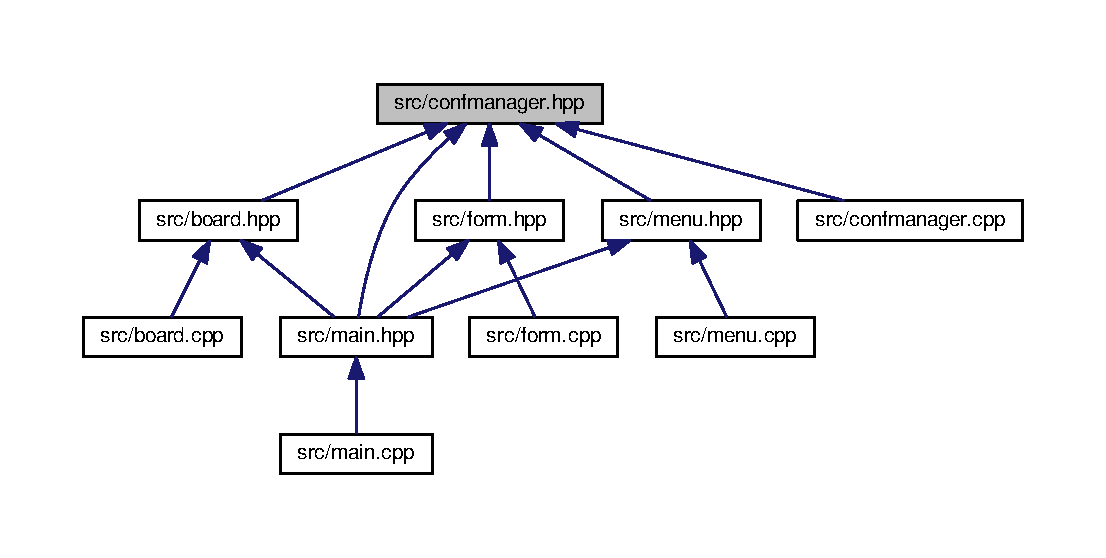
\includegraphics[width=350pt]{confmanager_8hpp__dep__incl}
\end{center}
\end{figure}
\subsection*{Macros}
\begin{DoxyCompactItemize}
\item 
\hypertarget{confmanager_8hpp_a3b34123ca1532b57b18493ad8d27d3ea}{\#define \hyperlink{confmanager_8hpp_a3b34123ca1532b57b18493ad8d27d3ea}{C\-O\-N\-F\-I\-G\-\_\-\-F\-I\-L\-E\-\_\-\-P\-A\-T\-H}~\char`\"{}config.\-cfg\char`\"{}}\label{confmanager_8hpp_a3b34123ca1532b57b18493ad8d27d3ea}

\begin{DoxyCompactList}\small\item\em The (relative) path of the config file at execution. \end{DoxyCompactList}\end{DoxyCompactItemize}
\subsection*{Functions}
\begin{DoxyCompactItemize}
\item 
{\footnotesize template$<$typename T\-Y\-P\-E $>$ }\\T\-Y\-P\-E \hyperlink{confmanager_8hpp_ab494c812df3bda0b52b01fc351dd02b5}{Read\-Variable} (const std\-::string \&K\-File\-Name, const std\-::string \&K\-Variable\-Name)
\begin{DoxyCompactList}\small\item\em Configuration file parser for one variable. \end{DoxyCompactList}\item 
{\footnotesize template$<$typename T\-Y\-P\-E $>$ }\\void \hyperlink{confmanager_8hpp_a4442b582c706ad30402a040866834f36}{Write\-Variable} (const std\-::string \&K\-File\-Name, const std\-::string \&K\-Variable\-Name, const T\-Y\-P\-E \&K\-Variable\-Value, bool Erase\-File)
\begin{DoxyCompactList}\small\item\em Configuration file writer for one variable. \end{DoxyCompactList}\item 
\hyperlink{common_8hpp_a3b27da0d46d4c36bc71511bcea2db296}{Player} \hyperlink{confmanager_8hpp_a7320e0a28c46c1cf87e5b1e37c4d118f}{Read\-Starting\-Player} ()
\begin{DoxyCompactList}\small\item\em Reads the starting Player in the config file. \end{DoxyCompactList}\item 
\hyperlink{common_8hpp_af5a69199868671fc85779715443d7e7d}{Coor} \hyperlink{confmanager_8hpp_a21454348fa3ef45b2521b40eccb565c1}{Read\-Board\-Dimensions} ()
\begin{DoxyCompactList}\small\item\em Reads the dimensions of the board in the config file. \end{DoxyCompactList}\item 
int \hyperlink{confmanager_8hpp_abed3527c8a74d39e07eca9b02fd76e4f}{Read\-Player\-Color} (\hyperlink{common_8hpp_a3b27da0d46d4c36bc71511bcea2db296}{Player} player)
\begin{DoxyCompactList}\small\item\em Reads the player color in the config file. \end{DoxyCompactList}\item 
int \hyperlink{confmanager_8hpp_ae91dc572702641134500948058bbfd8d}{Read\-Item\-Color} ()
\begin{DoxyCompactList}\small\item\em Reads the item color in the config file. \end{DoxyCompactList}\item 
float \hyperlink{confmanager_8hpp_a3d0fe9400c5579cf4c83a4df7c7dd210}{Read\-Barrier\-Apparition\-Frequency} ()
\begin{DoxyCompactList}\small\item\em Reads the apparition frequency of barriers. \end{DoxyCompactList}\item 
float \hyperlink{confmanager_8hpp_af93dd7fca974f94ff41fb678dd128be6}{Read\-Item\-Apparition\-Frequency} ()
\begin{DoxyCompactList}\small\item\em Reads the apparition frequency of items. \end{DoxyCompactList}\item 
bool \hyperlink{confmanager_8hpp_a372660ab9be4353c3edd6538e863ffd1}{Read\-Dots\-For\-Background} ()
\begin{DoxyCompactList}\small\item\em Read if the background display dots or not. \end{DoxyCompactList}\item 
void \hyperlink{confmanager_8hpp_a1d7e449f88cd4b8f3f304bffedff4cf8}{Write\-Float\-In\-File} (const std\-::string \&K\-Variable\-Name, char $\ast$Variable\-Value)
\begin{DoxyCompactList}\small\item\em Write a float number in the configuration file. \end{DoxyCompactList}\item 
void \hyperlink{confmanager_8hpp_aa77d65a36d86e37926c1c3accd5bcd4f}{Write\-Int\-In\-File} (const std\-::string \&K\-Variable\-Name, char $\ast$Variable\-Value)
\begin{DoxyCompactList}\small\item\em Write an integer number in the configuration file. \end{DoxyCompactList}\item 
void \hyperlink{confmanager_8hpp_a99faa18985acbb2d89b8c67a350ca1d0}{Write\-Comment\-In\-File} (const std\-::string \&K\-Comment, bool Erase\-File=false)
\begin{DoxyCompactList}\small\item\em Write a comment in the configuration file. \end{DoxyCompactList}\end{DoxyCompactItemize}


\subsection{Detailed Description}
Configuration file management header. \begin{DoxyAuthor}{Authors}
\-: J. Saffi, Y. Vidal, Y. Roux, A. Torres Aurora Dugo
\end{DoxyAuthor}
\begin{DoxyDate}{Date}
\-: 08/01/14
\end{DoxyDate}
\begin{DoxyVersion}{Version}
\-: 1.\-0
\end{DoxyVersion}
\begin{DoxySeeAlso}{See Also}
\hyperlink{confmanager_8cpp}{confmanager.\-cpp} 
\end{DoxySeeAlso}


\subsection{Function Documentation}
\hypertarget{confmanager_8hpp_a3d0fe9400c5579cf4c83a4df7c7dd210}{\index{confmanager.\-hpp@{confmanager.\-hpp}!Read\-Barrier\-Apparition\-Frequency@{Read\-Barrier\-Apparition\-Frequency}}
\index{Read\-Barrier\-Apparition\-Frequency@{Read\-Barrier\-Apparition\-Frequency}!confmanager.hpp@{confmanager.\-hpp}}
\subsubsection[{Read\-Barrier\-Apparition\-Frequency}]{\setlength{\rightskip}{0pt plus 5cm}float Read\-Barrier\-Apparition\-Frequency (
\begin{DoxyParamCaption}
{}
\end{DoxyParamCaption}
)}}\label{confmanager_8hpp_a3d0fe9400c5579cf4c83a4df7c7dd210}


Reads the apparition frequency of barriers. 

\begin{DoxyReturn}{Returns}
The apparition frequency of barriers.
\end{DoxyReturn}
The returned value is between 0 and 1. 

Here is the caller graph for this function\-:
\nopagebreak
\begin{figure}[H]
\begin{center}
\leavevmode
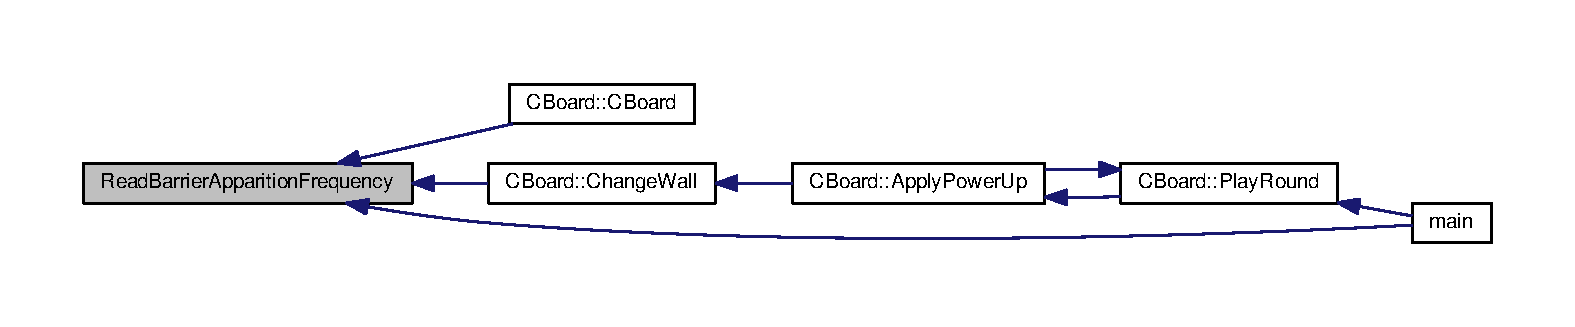
\includegraphics[width=350pt]{confmanager_8hpp_a3d0fe9400c5579cf4c83a4df7c7dd210_icgraph}
\end{center}
\end{figure}


\hypertarget{confmanager_8hpp_a21454348fa3ef45b2521b40eccb565c1}{\index{confmanager.\-hpp@{confmanager.\-hpp}!Read\-Board\-Dimensions@{Read\-Board\-Dimensions}}
\index{Read\-Board\-Dimensions@{Read\-Board\-Dimensions}!confmanager.hpp@{confmanager.\-hpp}}
\subsubsection[{Read\-Board\-Dimensions}]{\setlength{\rightskip}{0pt plus 5cm}{\bf Coor} Read\-Board\-Dimensions (
\begin{DoxyParamCaption}
{}
\end{DoxyParamCaption}
)}}\label{confmanager_8hpp_a21454348fa3ef45b2521b40eccb565c1}


Reads the dimensions of the board in the config file. 

\begin{DoxyReturn}{Returns}
The dimensions of the board.
\end{DoxyReturn}
The function will return the dimensions of the board as set in the configuration file. It uses the Read\-Variable function. The path of the config file is specified in a define made in \hyperlink{confmanager_8hpp}{confmanager.\-hpp} 

Here is the caller graph for this function\-:
\nopagebreak
\begin{figure}[H]
\begin{center}
\leavevmode
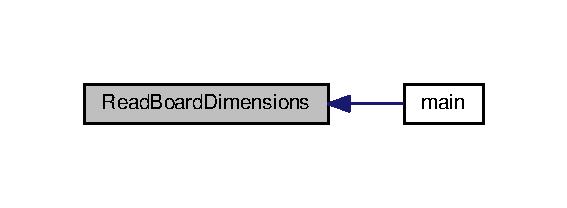
\includegraphics[width=272pt]{confmanager_8hpp_a21454348fa3ef45b2521b40eccb565c1_icgraph}
\end{center}
\end{figure}


\hypertarget{confmanager_8hpp_a372660ab9be4353c3edd6538e863ffd1}{\index{confmanager.\-hpp@{confmanager.\-hpp}!Read\-Dots\-For\-Background@{Read\-Dots\-For\-Background}}
\index{Read\-Dots\-For\-Background@{Read\-Dots\-For\-Background}!confmanager.hpp@{confmanager.\-hpp}}
\subsubsection[{Read\-Dots\-For\-Background}]{\setlength{\rightskip}{0pt plus 5cm}bool Read\-Dots\-For\-Background (
\begin{DoxyParamCaption}
{}
\end{DoxyParamCaption}
)}}\label{confmanager_8hpp_a372660ab9be4353c3edd6538e863ffd1}


Read if the background display dots or not. 

\begin{DoxyReturn}{Returns}
If the background has dots or not.
\end{DoxyReturn}
The returned value is a booleen that will set the background character to none or dots. 

Here is the caller graph for this function\-:
\nopagebreak
\begin{figure}[H]
\begin{center}
\leavevmode
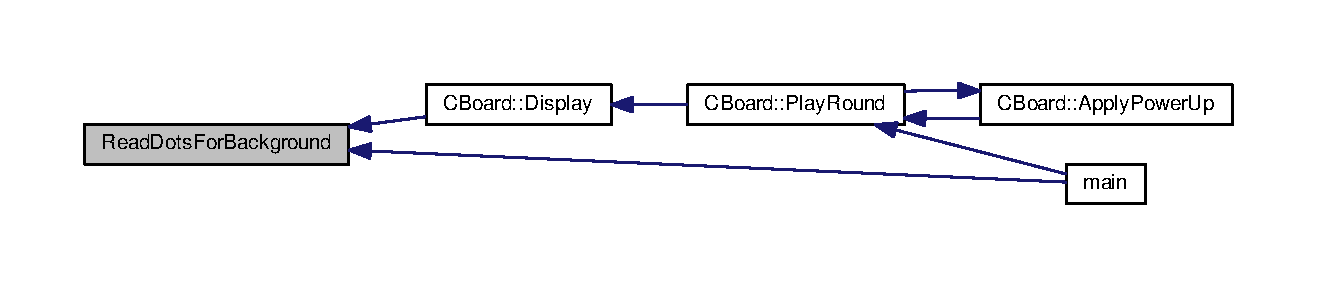
\includegraphics[width=350pt]{confmanager_8hpp_a372660ab9be4353c3edd6538e863ffd1_icgraph}
\end{center}
\end{figure}


\hypertarget{confmanager_8hpp_af93dd7fca974f94ff41fb678dd128be6}{\index{confmanager.\-hpp@{confmanager.\-hpp}!Read\-Item\-Apparition\-Frequency@{Read\-Item\-Apparition\-Frequency}}
\index{Read\-Item\-Apparition\-Frequency@{Read\-Item\-Apparition\-Frequency}!confmanager.hpp@{confmanager.\-hpp}}
\subsubsection[{Read\-Item\-Apparition\-Frequency}]{\setlength{\rightskip}{0pt plus 5cm}float Read\-Item\-Apparition\-Frequency (
\begin{DoxyParamCaption}
{}
\end{DoxyParamCaption}
)}}\label{confmanager_8hpp_af93dd7fca974f94ff41fb678dd128be6}


Reads the apparition frequency of items. 

\begin{DoxyReturn}{Returns}
The apparition frequency of items.
\end{DoxyReturn}
The returned value is between 0 and 1. 

Here is the caller graph for this function\-:
\nopagebreak
\begin{figure}[H]
\begin{center}
\leavevmode
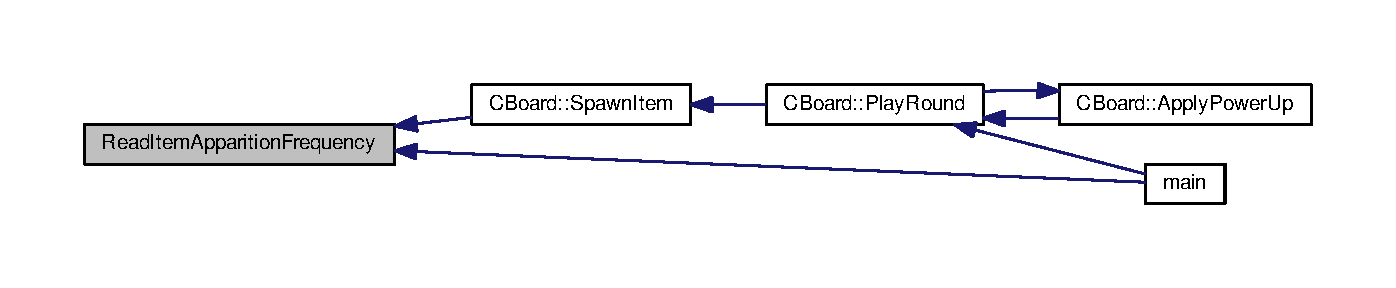
\includegraphics[width=350pt]{confmanager_8hpp_af93dd7fca974f94ff41fb678dd128be6_icgraph}
\end{center}
\end{figure}


\hypertarget{confmanager_8hpp_ae91dc572702641134500948058bbfd8d}{\index{confmanager.\-hpp@{confmanager.\-hpp}!Read\-Item\-Color@{Read\-Item\-Color}}
\index{Read\-Item\-Color@{Read\-Item\-Color}!confmanager.hpp@{confmanager.\-hpp}}
\subsubsection[{Read\-Item\-Color}]{\setlength{\rightskip}{0pt plus 5cm}int Read\-Item\-Color (
\begin{DoxyParamCaption}
{}
\end{DoxyParamCaption}
)}}\label{confmanager_8hpp_ae91dc572702641134500948058bbfd8d}


Reads the item color in the config file. 

\begin{DoxyReturn}{Returns}
The Item's color equivalent as an ncurses define.
\end{DoxyReturn}
It uses the Read\-Variable function to read the configuration file. The path of the config file is specified in a define made in \hyperlink{confmanager_8hpp}{confmanager.\-hpp} 

Here is the caller graph for this function\-:
\nopagebreak
\begin{figure}[H]
\begin{center}
\leavevmode
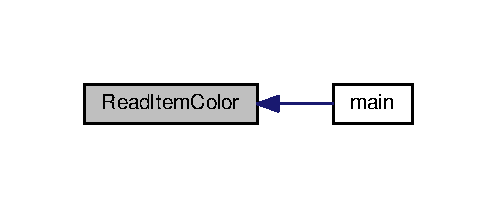
\includegraphics[width=238pt]{confmanager_8hpp_ae91dc572702641134500948058bbfd8d_icgraph}
\end{center}
\end{figure}


\hypertarget{confmanager_8hpp_abed3527c8a74d39e07eca9b02fd76e4f}{\index{confmanager.\-hpp@{confmanager.\-hpp}!Read\-Player\-Color@{Read\-Player\-Color}}
\index{Read\-Player\-Color@{Read\-Player\-Color}!confmanager.hpp@{confmanager.\-hpp}}
\subsubsection[{Read\-Player\-Color}]{\setlength{\rightskip}{0pt plus 5cm}int Read\-Player\-Color (
\begin{DoxyParamCaption}
\item[{{\bf Player}}]{player}
\end{DoxyParamCaption}
)}}\label{confmanager_8hpp_abed3527c8a74d39e07eca9b02fd76e4f}


Reads the player color in the config file. 


\begin{DoxyParams}{Parameters}
{\em player} & Player to get the color of. \\
\hline
\end{DoxyParams}
\begin{DoxyReturn}{Returns}
The Player's color equivalent as an ncurses define.
\end{DoxyReturn}
The function will return the color of the player whose name is the parameter. It uses the Read\-Variable function to read the configuration file. The path of the config file is specified in a define made in \hyperlink{confmanager_8hpp}{confmanager.\-hpp} 

Here is the caller graph for this function\-:
\nopagebreak
\begin{figure}[H]
\begin{center}
\leavevmode
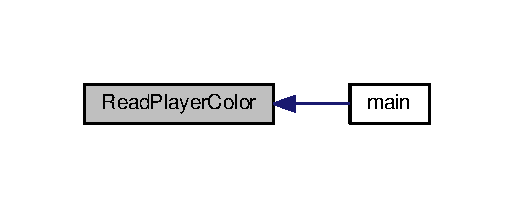
\includegraphics[width=246pt]{confmanager_8hpp_abed3527c8a74d39e07eca9b02fd76e4f_icgraph}
\end{center}
\end{figure}


\hypertarget{confmanager_8hpp_a7320e0a28c46c1cf87e5b1e37c4d118f}{\index{confmanager.\-hpp@{confmanager.\-hpp}!Read\-Starting\-Player@{Read\-Starting\-Player}}
\index{Read\-Starting\-Player@{Read\-Starting\-Player}!confmanager.hpp@{confmanager.\-hpp}}
\subsubsection[{Read\-Starting\-Player}]{\setlength{\rightskip}{0pt plus 5cm}{\bf Player} Read\-Starting\-Player (
\begin{DoxyParamCaption}
{}
\end{DoxyParamCaption}
)}}\label{confmanager_8hpp_a7320e0a28c46c1cf87e5b1e37c4d118f}


Reads the starting Player in the config file. 

\begin{DoxyReturn}{Returns}
The starting Player.
\end{DoxyReturn}
The function will return which player will begin to play. It uses the Read\-Variable Function. The path of the config file is specified in a define made in \hyperlink{confmanager_8hpp}{confmanager.\-hpp} 

Here is the caller graph for this function\-:
\nopagebreak
\begin{figure}[H]
\begin{center}
\leavevmode
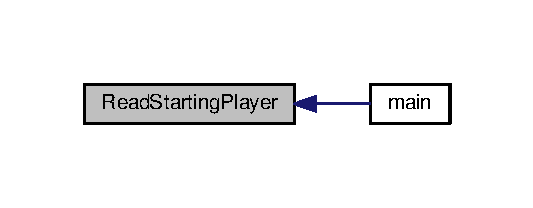
\includegraphics[width=256pt]{confmanager_8hpp_a7320e0a28c46c1cf87e5b1e37c4d118f_icgraph}
\end{center}
\end{figure}


\hypertarget{confmanager_8hpp_ab494c812df3bda0b52b01fc351dd02b5}{\index{confmanager.\-hpp@{confmanager.\-hpp}!Read\-Variable@{Read\-Variable}}
\index{Read\-Variable@{Read\-Variable}!confmanager.hpp@{confmanager.\-hpp}}
\subsubsection[{Read\-Variable}]{\setlength{\rightskip}{0pt plus 5cm}template$<$typename T\-Y\-P\-E $>$ T\-Y\-P\-E Read\-Variable (
\begin{DoxyParamCaption}
\item[{const std\-::string \&}]{K\-File\-Name, }
\item[{const std\-::string \&}]{K\-Variable\-Name}
\end{DoxyParamCaption}
)}}\label{confmanager_8hpp_ab494c812df3bda0b52b01fc351dd02b5}


Configuration file parser for one variable. 


\begin{DoxyParams}{Parameters}
{\em K\-File\-Name} & File path of the configuration file. \\
\hline
{\em K\-Variable\-Name} & Name of the parsed variable. \\
\hline
\end{DoxyParams}
\begin{DoxyReturn}{Returns}
The parsed value of the variable.
\end{DoxyReturn}
The function will parse the file we give him in first place parameter. To achieve this, it will read the variable's value in the configuration file and return the value. It uses a template to be able to parse any type using operator $>$$>$ \hypertarget{confmanager_8hpp_a99faa18985acbb2d89b8c67a350ca1d0}{\index{confmanager.\-hpp@{confmanager.\-hpp}!Write\-Comment\-In\-File@{Write\-Comment\-In\-File}}
\index{Write\-Comment\-In\-File@{Write\-Comment\-In\-File}!confmanager.hpp@{confmanager.\-hpp}}
\subsubsection[{Write\-Comment\-In\-File}]{\setlength{\rightskip}{0pt plus 5cm}void Write\-Comment\-In\-File (
\begin{DoxyParamCaption}
\item[{const std\-::string \&}]{K\-Comment, }
\item[{bool}]{Erase\-File}
\end{DoxyParamCaption}
)}}\label{confmanager_8hpp_a99faa18985acbb2d89b8c67a350ca1d0}


Write a comment in the configuration file. 


\begin{DoxyParams}{Parameters}
{\em K\-Comment} & The comment to inject. \\
\hline
{\em Erase\-File} & Set if the configuration file have to be erased.\\
\hline
\end{DoxyParams}
The function will write the the comment gave in parameters thanks to the Write\-Variable template 

Here is the caller graph for this function\-:
\nopagebreak
\begin{figure}[H]
\begin{center}
\leavevmode
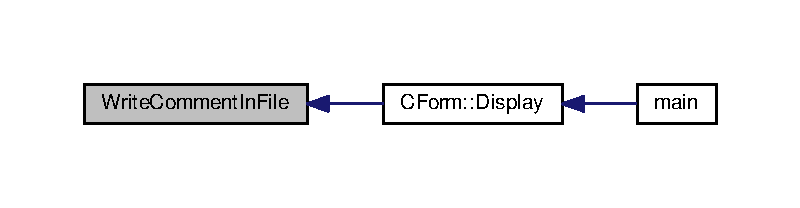
\includegraphics[width=350pt]{confmanager_8hpp_a99faa18985acbb2d89b8c67a350ca1d0_icgraph}
\end{center}
\end{figure}


\hypertarget{confmanager_8hpp_a1d7e449f88cd4b8f3f304bffedff4cf8}{\index{confmanager.\-hpp@{confmanager.\-hpp}!Write\-Float\-In\-File@{Write\-Float\-In\-File}}
\index{Write\-Float\-In\-File@{Write\-Float\-In\-File}!confmanager.hpp@{confmanager.\-hpp}}
\subsubsection[{Write\-Float\-In\-File}]{\setlength{\rightskip}{0pt plus 5cm}void Write\-Float\-In\-File (
\begin{DoxyParamCaption}
\item[{const std\-::string \&}]{K\-Variable\-Name, }
\item[{char $\ast$}]{Variable\-Value}
\end{DoxyParamCaption}
)}}\label{confmanager_8hpp_a1d7e449f88cd4b8f3f304bffedff4cf8}


Write a float number in the configuration file. 


\begin{DoxyParams}{Parameters}
{\em K\-Variable\-Name} & The name of the variable to inject. \\
\hline
{\em Variable\-Value} & The value of the variable to inject.\\
\hline
\end{DoxyParams}
The function will write the name of the float variable and her value thanks to the Write\-Variable template. 

Here is the caller graph for this function\-:
\nopagebreak
\begin{figure}[H]
\begin{center}
\leavevmode
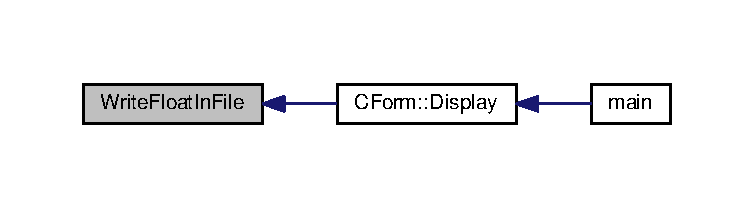
\includegraphics[width=350pt]{confmanager_8hpp_a1d7e449f88cd4b8f3f304bffedff4cf8_icgraph}
\end{center}
\end{figure}


\hypertarget{confmanager_8hpp_aa77d65a36d86e37926c1c3accd5bcd4f}{\index{confmanager.\-hpp@{confmanager.\-hpp}!Write\-Int\-In\-File@{Write\-Int\-In\-File}}
\index{Write\-Int\-In\-File@{Write\-Int\-In\-File}!confmanager.hpp@{confmanager.\-hpp}}
\subsubsection[{Write\-Int\-In\-File}]{\setlength{\rightskip}{0pt plus 5cm}void Write\-Int\-In\-File (
\begin{DoxyParamCaption}
\item[{const std\-::string \&}]{K\-Variable\-Name, }
\item[{char $\ast$}]{Variable\-Value}
\end{DoxyParamCaption}
)}}\label{confmanager_8hpp_aa77d65a36d86e37926c1c3accd5bcd4f}


Write an integer number in the configuration file. 


\begin{DoxyParams}{Parameters}
{\em K\-Variable\-Name} & Name of the variable to inject. \\
\hline
{\em Variable\-Value} & Value of the variable to inject.\\
\hline
\end{DoxyParams}
The function will write the name of the integer variable and her value thanks to the Write\-Variable template. 

Here is the caller graph for this function\-:
\nopagebreak
\begin{figure}[H]
\begin{center}
\leavevmode
\includegraphics[width=350pt]{confmanager_8hpp_aa77d65a36d86e37926c1c3accd5bcd4f_icgraph}
\end{center}
\end{figure}


\hypertarget{confmanager_8hpp_a4442b582c706ad30402a040866834f36}{\index{confmanager.\-hpp@{confmanager.\-hpp}!Write\-Variable@{Write\-Variable}}
\index{Write\-Variable@{Write\-Variable}!confmanager.hpp@{confmanager.\-hpp}}
\subsubsection[{Write\-Variable}]{\setlength{\rightskip}{0pt plus 5cm}template$<$typename T\-Y\-P\-E $>$ void Write\-Variable (
\begin{DoxyParamCaption}
\item[{const std\-::string \&}]{K\-File\-Name, }
\item[{const std\-::string \&}]{K\-Variable\-Name, }
\item[{const T\-Y\-P\-E \&}]{K\-Variable\-Value, }
\item[{bool}]{Erase\-File}
\end{DoxyParamCaption}
)}}\label{confmanager_8hpp_a4442b582c706ad30402a040866834f36}


Configuration file writer for one variable. 


\begin{DoxyParams}{Parameters}
{\em K\-File\-Name} & File path of the configuration file. \\
\hline
{\em K\-Variable\-Name} & Name of the variable to inject. \\
\hline
{\em K\-Variable\-Value} & Value of the variable to inject. \\
\hline
{\em Erase\-File} & Set if the file must be erased before being writed.\\
\hline
\end{DoxyParams}
The function will write the file we give him in first place parameter and her value we give in second place parameter. To achieve this, it will write the variable and then value in the configuration file. It uses a template to be able to write any type properly using operator $>$$>$ 
\hypertarget{form_8cpp}{\section{src/form.cpp File Reference}
\label{form_8cpp}\index{src/form.\-cpp@{src/form.\-cpp}}
}


Implementation of the Form class.  


{\ttfamily \#include \char`\"{}form.\-hpp\char`\"{}}\\*
Include dependency graph for form.\-cpp\-:
\nopagebreak
\begin{figure}[H]
\begin{center}
\leavevmode
\includegraphics[width=350pt]{form_8cpp__incl}
\end{center}
\end{figure}


\subsection{Detailed Description}
Implementation of the Form class. \begin{DoxyAuthor}{Authors}
\-: J. Saffi, Y. Vidal, Y. Roux, A. Torres Aurora Dugo
\end{DoxyAuthor}
\begin{DoxyDate}{Date}
\-: 08/01/14
\end{DoxyDate}
\begin{DoxyVersion}{Version}
\-: 1.\-0
\end{DoxyVersion}
\begin{DoxySeeAlso}{See Also}
\hyperlink{form_8hpp}{form.\-hpp} 
\end{DoxySeeAlso}

\hypertarget{form_8hpp}{\section{src/form.hpp File Reference}
\label{form_8hpp}\index{src/form.\-hpp@{src/form.\-hpp}}
}


Header of the Form class.  


{\ttfamily \#include \char`\"{}confmanager.\-hpp\char`\"{}}\\*
{\ttfamily \#include $<$vector$>$}\\*
{\ttfamily \#include $<$form.\-h$>$}\\*
{\ttfamily \#include $<$fstream$>$}\\*
{\ttfamily \#include $<$stdexcept$>$}\\*
{\ttfamily \#include $<$exception$>$}\\*
{\ttfamily \#include $<$ncurses.\-h$>$}\\*
Include dependency graph for form.\-hpp\-:
\nopagebreak
\begin{figure}[H]
\begin{center}
\leavevmode
\includegraphics[width=350pt]{form_8hpp__incl}
\end{center}
\end{figure}
This graph shows which files directly or indirectly include this file\-:
\nopagebreak
\begin{figure}[H]
\begin{center}
\leavevmode
\includegraphics[width=241pt]{form_8hpp__dep__incl}
\end{center}
\end{figure}
\subsection*{Classes}
\begin{DoxyCompactItemize}
\item 
class \hyperlink{class_c_form}{C\-Form}
\begin{DoxyCompactList}\small\item\em The form used as settings panel. \end{DoxyCompactList}\end{DoxyCompactItemize}


\subsection{Detailed Description}
Header of the Form class. \begin{DoxyAuthor}{Authors}
\-: J. Saffi, Y. Vidal, Y. Roux, A. Torres Aurora Dugo
\end{DoxyAuthor}
\begin{DoxyDate}{Date}
\-: 08/01/14
\end{DoxyDate}
\begin{DoxyVersion}{Version}
\-: 1.\-0
\end{DoxyVersion}
\begin{DoxySeeAlso}{See Also}
\hyperlink{form_8cpp}{form.\-cpp} 
\end{DoxySeeAlso}

\hypertarget{help_8cpp}{\section{src/help.cpp File Reference}
\label{help_8cpp}\index{src/help.\-cpp@{src/help.\-cpp}}
}


Help display implementation.  


{\ttfamily \#include \char`\"{}help.\-hpp\char`\"{}}\\*
Include dependency graph for help.\-cpp\-:
\nopagebreak
\begin{figure}[H]
\begin{center}
\leavevmode
\includegraphics[width=350pt]{help_8cpp__incl}
\end{center}
\end{figure}


\subsection{Detailed Description}
Help display implementation. \begin{DoxyAuthor}{Authors}
\-: J. Saffi, Y. Vidal, Y. Roux, A. Torres Aurora Dugo
\end{DoxyAuthor}
\begin{DoxyDate}{Date}
\-: 08/01/14
\end{DoxyDate}
\begin{DoxyVersion}{Version}
\-: 1.\-0
\end{DoxyVersion}
\begin{DoxySeeAlso}{See Also}
\hyperlink{help_8hpp}{help.\-hpp} 
\end{DoxySeeAlso}

\hypertarget{help_8hpp}{\section{src/help.hpp File Reference}
\label{help_8hpp}\index{src/help.\-hpp@{src/help.\-hpp}}
}


Help class header.  


{\ttfamily \#include \char`\"{}common.\-hpp\char`\"{}}\\*
{\ttfamily \#include $<$vector$>$}\\*
{\ttfamily \#include $<$fstream$>$}\\*
{\ttfamily \#include $<$stdexcept$>$}\\*
{\ttfamily \#include $<$exception$>$}\\*
{\ttfamily \#include $<$ncurses.\-h$>$}\\*
{\ttfamily \#include $<$iostream$>$}\\*
Include dependency graph for help.\-hpp\-:
\nopagebreak
\begin{figure}[H]
\begin{center}
\leavevmode
\includegraphics[width=350pt]{help_8hpp__incl}
\end{center}
\end{figure}
This graph shows which files directly or indirectly include this file\-:
\nopagebreak
\begin{figure}[H]
\begin{center}
\leavevmode
\includegraphics[width=241pt]{help_8hpp__dep__incl}
\end{center}
\end{figure}
\subsection*{Classes}
\begin{DoxyCompactItemize}
\item 
class \hyperlink{class_c_help}{C\-Help}
\begin{DoxyCompactList}\small\item\em The help window. \end{DoxyCompactList}\end{DoxyCompactItemize}
\subsection*{Macros}
\begin{DoxyCompactItemize}
\item 
\hypertarget{help_8hpp_a4911dec4cafe4d6fec850c8c84a0b80d}{\#define \hyperlink{help_8hpp_a4911dec4cafe4d6fec850c8c84a0b80d}{H\-E\-L\-P\-\_\-\-F\-I\-L\-E\-\_\-\-P\-A\-T\-H}~\char`\"{}help.\-txt\char`\"{}}\label{help_8hpp_a4911dec4cafe4d6fec850c8c84a0b80d}

\begin{DoxyCompactList}\small\item\em The (relative) path of the help file at execution. \end{DoxyCompactList}\end{DoxyCompactItemize}


\subsection{Detailed Description}
Help class header. \begin{DoxyAuthor}{Authors}
\-: J. Saffi, Y. Vidal, Y. Roux, A. Torres Aurora Dugo
\end{DoxyAuthor}
\begin{DoxyDate}{Date}
\-: 08/01/14
\end{DoxyDate}
\begin{DoxyVersion}{Version}
\-: 1.\-0
\end{DoxyVersion}
\begin{DoxySeeAlso}{See Also}
\hyperlink{help_8cpp}{help.\-cpp} 
\end{DoxySeeAlso}

\hypertarget{main_8cpp}{\section{src/main.cpp File Reference}
\label{main_8cpp}\index{src/main.\-cpp@{src/main.\-cpp}}
}


Main file.  


{\ttfamily \#include \char`\"{}main.\-hpp\char`\"{}}\\*
Include dependency graph for main.\-cpp\-:
\nopagebreak
\begin{figure}[H]
\begin{center}
\leavevmode
\includegraphics[width=350pt]{main_8cpp__incl}
\end{center}
\end{figure}
\subsection*{Functions}
\begin{DoxyCompactItemize}
\item 
\hypertarget{main_8cpp_ae66f6b31b5ad750f1fe042a706a4e3d4}{int \hyperlink{main_8cpp_ae66f6b31b5ad750f1fe042a706a4e3d4}{main} ()}\label{main_8cpp_ae66f6b31b5ad750f1fe042a706a4e3d4}

\begin{DoxyCompactList}\small\item\em Main function. \end{DoxyCompactList}\end{DoxyCompactItemize}


\subsection{Detailed Description}
Main file. \begin{DoxyAuthor}{Authors}
\-: J.\-Saffi, Y.\-Vidal, Y.\-Roux, A.\-Torres Aurora
\end{DoxyAuthor}
\begin{DoxyDate}{Date}
\-: 08/01/14
\end{DoxyDate}
\begin{DoxyVersion}{Version}
\-: 1.\-0
\end{DoxyVersion}
\begin{DoxySeeAlso}{See Also}
\hyperlink{main_8hpp}{main.\-hpp} 
\end{DoxySeeAlso}

\hypertarget{main_8hpp}{\section{src/main.hpp File Reference}
\label{main_8hpp}\index{src/main.\-hpp@{src/main.\-hpp}}
}


Main file header.  


{\ttfamily \#include \char`\"{}common.\-hpp\char`\"{}}\\*
{\ttfamily \#include \char`\"{}board.\-hpp\char`\"{}}\\*
{\ttfamily \#include \char`\"{}confmanager.\-hpp\char`\"{}}\\*
{\ttfamily \#include \char`\"{}menu.\-hpp\char`\"{}}\\*
{\ttfamily \#include \char`\"{}form.\-hpp\char`\"{}}\\*
{\ttfamily \#include \char`\"{}help.\-hpp\char`\"{}}\\*
{\ttfamily \#include $<$cstdlib$>$}\\*
{\ttfamily \#include $<$ncurses.\-h$>$}\\*
{\ttfamily \#include $<$iostream$>$}\\*
{\ttfamily \#include $<$chrono$>$}\\*
{\ttfamily \#include $<$thread$>$}\\*
Include dependency graph for main.\-hpp\-:
\nopagebreak
\begin{figure}[H]
\begin{center}
\leavevmode
\includegraphics[width=350pt]{main_8hpp__incl}
\end{center}
\end{figure}
This graph shows which files directly or indirectly include this file\-:
\nopagebreak
\begin{figure}[H]
\begin{center}
\leavevmode
\includegraphics[width=152pt]{main_8hpp__dep__incl}
\end{center}
\end{figure}


\subsection{Detailed Description}
Main file header. \begin{DoxyAuthor}{Authors}
\-: J. Saffi, Y. Vidal, Y. Roux, A. Torres Aurora Dugo
\end{DoxyAuthor}
\begin{DoxyDate}{Date}
\-: 08/01/14
\end{DoxyDate}
\begin{DoxyVersion}{Version}
\-: 1.\-0
\end{DoxyVersion}
\begin{DoxySeeAlso}{See Also}
\hyperlink{main_8cpp}{main.\-cpp} 
\end{DoxySeeAlso}

\hypertarget{menu_8cpp}{\section{src/menu.cpp File Reference}
\label{menu_8cpp}\index{src/menu.\-cpp@{src/menu.\-cpp}}
}


Menu class implementation.  


{\ttfamily \#include \char`\"{}menu.\-hpp\char`\"{}}\\*
Include dependency graph for menu.\-cpp\-:
\nopagebreak
\begin{figure}[H]
\begin{center}
\leavevmode
\includegraphics[width=350pt]{menu_8cpp__incl}
\end{center}
\end{figure}


\subsection{Detailed Description}
Menu class implementation. \begin{DoxyAuthor}{Authors}
\-: J. Saffi, Y. Vidal, Y. Roux, A. Torres Aurora Dugo
\end{DoxyAuthor}
\begin{DoxyDate}{Date}
\-: 08/01/14
\end{DoxyDate}
\begin{DoxyVersion}{Version}
\-: 1.\-0
\end{DoxyVersion}
\begin{DoxySeeAlso}{See Also}
\hyperlink{menu_8hpp}{menu.\-hpp} 
\end{DoxySeeAlso}

\hypertarget{menu_8hpp}{\section{src/menu.hpp File Reference}
\label{menu_8hpp}\index{src/menu.\-hpp@{src/menu.\-hpp}}
}


Menu class header.  


{\ttfamily \#include \char`\"{}common.\-hpp\char`\"{}}\\*
{\ttfamily \#include \char`\"{}confmanager.\-hpp\char`\"{}}\\*
{\ttfamily \#include $<$ncurses.\-h$>$}\\*
{\ttfamily \#include $<$menu.\-h$>$}\\*
{\ttfamily \#include $<$exception$>$}\\*
{\ttfamily \#include $<$vector$>$}\\*
{\ttfamily \#include $<$string$>$}\\*
Include dependency graph for menu.\-hpp\-:
\nopagebreak
\begin{figure}[H]
\begin{center}
\leavevmode
\includegraphics[width=350pt]{menu_8hpp__incl}
\end{center}
\end{figure}
This graph shows which files directly or indirectly include this file\-:
\nopagebreak
\begin{figure}[H]
\begin{center}
\leavevmode
\includegraphics[width=247pt]{menu_8hpp__dep__incl}
\end{center}
\end{figure}
\subsection*{Classes}
\begin{DoxyCompactItemize}
\item 
class \hyperlink{class_c_menu}{C\-Menu}
\begin{DoxyCompactList}\small\item\em A user-\/friendly menu. \end{DoxyCompactList}\end{DoxyCompactItemize}


\subsection{Detailed Description}
Menu class header. \begin{DoxyAuthor}{Authors}
\-: J. Saffi, Y. Vidal, Y. Roux, A. Torres Aurora Dugo
\end{DoxyAuthor}
\begin{DoxyDate}{Date}
\-: 08/01/14
\end{DoxyDate}
\begin{DoxyVersion}{Version}
\-: 1.\-0
\end{DoxyVersion}
\begin{DoxySeeAlso}{See Also}
\hyperlink{menu_8cpp}{menu.\-cpp} 
\end{DoxySeeAlso}

\hypertarget{square_8cpp}{\section{src/square.cpp File Reference}
\label{square_8cpp}\index{src/square.\-cpp@{src/square.\-cpp}}
}


Square class implementation.  


{\ttfamily \#include \char`\"{}square.\-hpp\char`\"{}}\\*
Include dependency graph for square.\-cpp\-:
\nopagebreak
\begin{figure}[H]
\begin{center}
\leavevmode
\includegraphics[width=306pt]{square_8cpp__incl}
\end{center}
\end{figure}


\subsection{Detailed Description}
Square class implementation. \begin{DoxyAuthor}{Authors}
\-: J. Saffi, Y. Vidal, Y. Roux, A. Torres Aurora Dugo
\end{DoxyAuthor}
\begin{DoxyDate}{Date}
\-: 08/01/14
\end{DoxyDate}
\begin{DoxyVersion}{Version}
\-: 1.\-0
\end{DoxyVersion}
\begin{DoxySeeAlso}{See Also}
\hyperlink{square_8hpp}{square.\-hpp} 
\end{DoxySeeAlso}

\hypertarget{square_8hpp}{\section{src/square.hpp File Reference}
\label{square_8hpp}\index{src/square.\-hpp@{src/square.\-hpp}}
}


Square class header.  


{\ttfamily \#include \char`\"{}common.\-hpp\char`\"{}}\\*
{\ttfamily \#include $<$exception$>$}\\*
{\ttfamily \#include $<$stdexcept$>$}\\*
Include dependency graph for square.\-hpp\-:
\nopagebreak
\begin{figure}[H]
\begin{center}
\leavevmode
\includegraphics[width=306pt]{square_8hpp__incl}
\end{center}
\end{figure}
This graph shows which files directly or indirectly include this file\-:
\nopagebreak
\begin{figure}[H]
\begin{center}
\leavevmode
\includegraphics[width=301pt]{square_8hpp__dep__incl}
\end{center}
\end{figure}
\subsection*{Classes}
\begin{DoxyCompactItemize}
\item 
class \hyperlink{class_c_square}{C\-Square}
\begin{DoxyCompactList}\small\item\em The squares of the board. \end{DoxyCompactList}\end{DoxyCompactItemize}


\subsection{Detailed Description}
Square class header. \begin{DoxyAuthor}{Authors}
\-: J. Saffi, Y. Vidal, Y. Roux, A. Torres Aurora Dugo
\end{DoxyAuthor}
\begin{DoxyDate}{Date}
\-: 08/01/14
\end{DoxyDate}
\begin{DoxyVersion}{Version}
\-: 1.\-0
\end{DoxyVersion}
\begin{DoxySeeAlso}{See Also}
\hyperlink{square_8cpp}{square.\-cpp} 
\end{DoxySeeAlso}

%--- End generated contents ---

% Index
\newpage
\phantomsection
\addcontentsline{toc}{chapter}{Index}
\printindex

\end{document}
